\documentclass{article}

\usepackage[top=2.5cm,left=2.5cm,right=2.5cm,bottom=2.5cm]{geometry}
\usepackage[utf8]{inputenc}
\usepackage[T1]{fontenc}
\usepackage[french]{babel}
\usepackage{graphicx}
\usepackage{multicol}
\usepackage{pdflscape}
\usepackage[pdfborder={0 0 0}]{hyperref}

\title{
\includegraphics{img/logo.png}\vspace{2cm}\\
    Stage chez Let There Be Light \\
    \large Rapport de stage Exia A4}

\date{24 Mars 2018}

\author{Stagiaire : Baptiste \bsc{Saclier} \\
    Maître de stage : Benjamin \bsc{Petit}\\
    Pilote de formation : Julio \bsc{Santilario}}

\begin{document}

    \maketitle

    \clearpage

    \tableofcontents

    \section{Introduction}

    Dans le cadre de ma 3\up{e} année au CESI EXiA, j'éfféctue actuellement un stage chez Let There Be Light.
    Cette entreprise réalise des dispositifs interactifs pour l'événementiel, la communication et la culture.

    Ce rapport relate de cette entreprise et des projets sur lesquels j'ai travaillé.

    \clearpage

    \section{Let There Be Light}

La société Let There Be Light (ou LTBL) est une société qui réalise des dispositifs interactifs pour l'événementiel, la communication et la culture.
Elle fut fondée en 2014 par Benjamin \bsc{Petit} et Antoine \bsc{Vanel} sous le nom de Beam'Art.
En 2016, elle change de nom et de statut pour devenir l'entreprise que l'on connaît aujourd'hui.
Actuellement, M. \bsc{Petit} en est le seul dirigeant et emploi 2 personnes.

\begin{description}
    \item[2012] Première fête des Lumières de Lyon dans le cadre d'une association avec un spectacle interactif nommé "Hypermétrope"
    \item[2014] Fondation de la société Beam'Art
    \item[2014] Installation interactive "Hi Striker" sur le palais de justice
    \item[2014] Mapping "TranJS" à Bernes
    \item[2015] Installation interactive "Lumibus" pour Keolis
    \item[2016] Changement de nom pour devenir Let There Be Light
    \item[2016] Participation à la création du showroom Pavillon de l'innovation pour Michelin
    \item[2017] Scénographie au Transbordeurs "DELete"
\end{description}

\subsection{Structure}

Let There Be Light est un partenaire de la société Vendredi 4.
Vendredi 4 est une société de communication spécialisée dans l'interaction.
Les contrats sont obtenus par Sylvie \bsc{Madamour}, la charte graphique du projet est alors composée par Vendredi 4.
LTBL intervient sur l'intégration de cette charte graphique dans les installations interactives dans des salons ou des showrooms.

Les équipes de Vendredi 4 et de LTBL sont assez réduites.
L'effectif de Vendredi 4 est de 3 employé quand LTBL compte un unique employé (Benjamin \bsc{Petit}) et deux consultants : Corentin \bsc{Limoge} et Alexander \bsc{Feller}.

\begin{figure}[h]
    \centering
    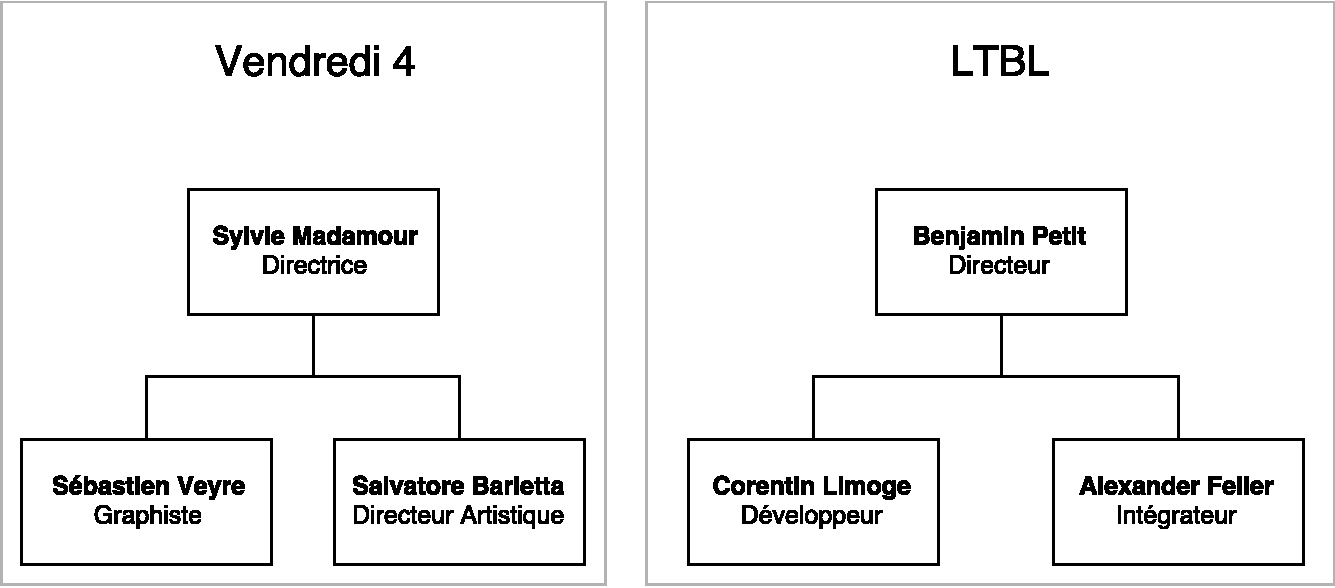
\includegraphics[scale=0.7]{img/Structure-LTBL.pdf}
    \caption{Structure de LTBL et Vendredi 4}
\end{figure}

Les deux entreprises sont très liées, elles partagent les mêmes locaux et communiquent beaucoup ensemble sur les projets en cours et à venir.

On retrouve alors Benjamin \bsc{Petit}, le gérant, et Corentin \bsc{Limoge} du côté LTBL.
Benjamin s'occupe des conseils et de la gestion de l'entreprise.
Il s'occupe aussi de l'aspect technique des installations par le choix des technologies de pointage et d'affichage.
Corentin est employé par LTBL, mais dispose d'un statut d'auto-entrepreneur, on peut alors le considérer comme un consultant.
Corentin est en charge du développement des applications qui seront exécutées sur les installations.

Du côté Vendredi 4, on retrouve Sylvie \bsc{Madamour}, la directrice, Salvatore \bsc{Barletta}, directeur artistique, et Sébastien \bsc{Veyre}, graphiste.
Sylvie est en charge des contrats, devis et de la communication avec les clients.
Salvatore est directeur artistique chez Vendredi 4, il s'occupe de concevoir et présenter les design des installations aux clients.
Sébastien est graphiste et est en charge de représenter les futures interfaces des installations, mais aussi de travailler sur des rendus en Motion Design\footnote{Une technique d'animation graphique ayant pour but de mettre en valeur le mouvement et l'animation.} Pour donner un premier aperçu de la future application pour les clients et les intégrateurs.

\subsection{Projets}

Les deux entreprises travaillent ensemble pour proposer des services suivants :

\begin{itemize}
    \item Conseils techniques
    \item Conseils en interaction
    \item Design graphique
    \item Développement d'applications interactives
    \item Installations
\end{itemize}

Ainsi, les deux entreprises peuvent suivre la production d'une application interactive de sa conception jusqu'à son installation.

\medskip

Les projets suivis par LTBL sont les suivants :

\paragraph{Dispositifs de présentation interactifs} le plus souvent utilisés dans les salons et showrooms, les dispositifs interactifs permettent une présentation des produits de manière esthétique.
L'objectif de LTBL est donc de concevoir cette installation.
Cela passe par la conception du système physique est des composants requis mais aussi par la conception et le développement de l'interface utilisateur qui doit être réactive et esthétique.
La majorité de ce type de projet est la présentation d'informations sur un produit sur un écran tactile

\paragraph{Vidéo Mapping} Le plus souvent présenté lors d'événements, le vidéo mapping consiste en la projection d'une image déformée sur une structure pouvant être un bâtiment ou une installation spécifique.
Cette image utilise une représentation de la structure pour se déformer et épouser sa forme lors de la projection.
Ce type d'installation permet, au travers de jeux de lumière et d'illusions, de donner vie à la structure ou au bâtiment.
On retrouve ce type d'installation à la fête des Lumières de Lyon par exemple.

\paragraph{Conseils techniques ou en interaction} Fort de son expérience dans le domaine de l'interactivité, LTBL peut aussi donner des conseils en interactivité dans le cadre de projets cités plus haut.

\paragraph{Fête des Lumières} La fête des Lumières est une manifestation Lyonnaise prenant place aux endroits importants de la ville.
Cette fête met en lumière de nombreuses installations lumineuses et interactives.
Chaque année, LTBL peut proposer un projet d'installation en rapport avec un bâtiment de la ville sur lequel s'installer.
Ce projet est alors évalué et est accepté ou non en fonction de la faisabilité, l'esthétique et le coût de l'installation.
La dernière fête des Lumières à laquelle a participé LTBL fut celle de 2015 avec une installation nommée "Lumibus".
Cette installation présentait un Bus muni de panneaux LED réagissant aux accélérations et freinages de celui-ci.
Les années précédentes, LTBL a aussi présenté Hi Striker, une installation reprenant le jeu de foire de la massue où les participants doivent taper le plus fort possible sur un capteur à l'aide d'une massue.
Plus la frappe est forte plus le bâtiment s'illumine.
Cette installation se trouvait au palais de justice.
Plus récemment, LTBL a participé à la fête des Lumières de Hong Kong avec un projet reprenant le même principe, mais en animant un dragon.

\begin{figure}[h]
    \centering
    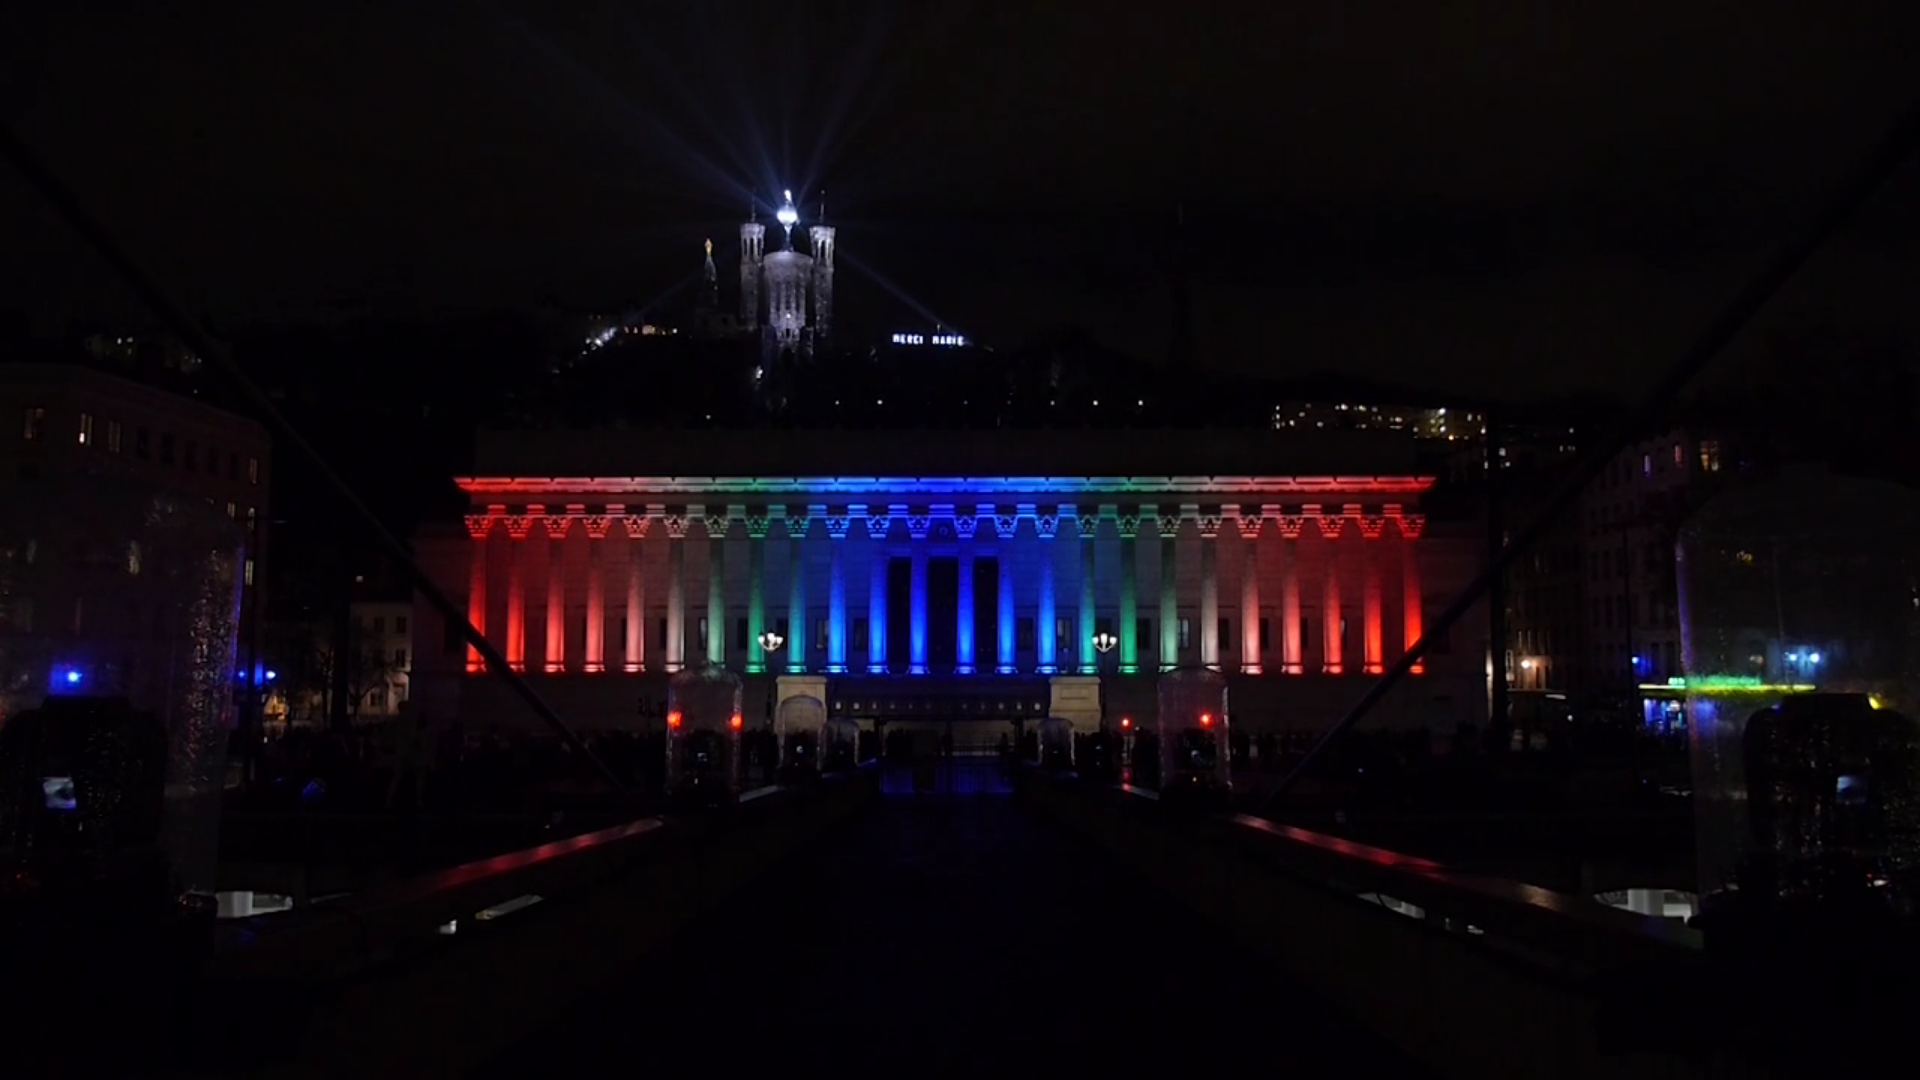
\includegraphics[scale=0.2]{img/hi-striker.png}
    \caption{L'installation "Hi Striker" à la fête des Lumières de Lyon}
\end{figure}


\begin{figure}[h]
    \centering
    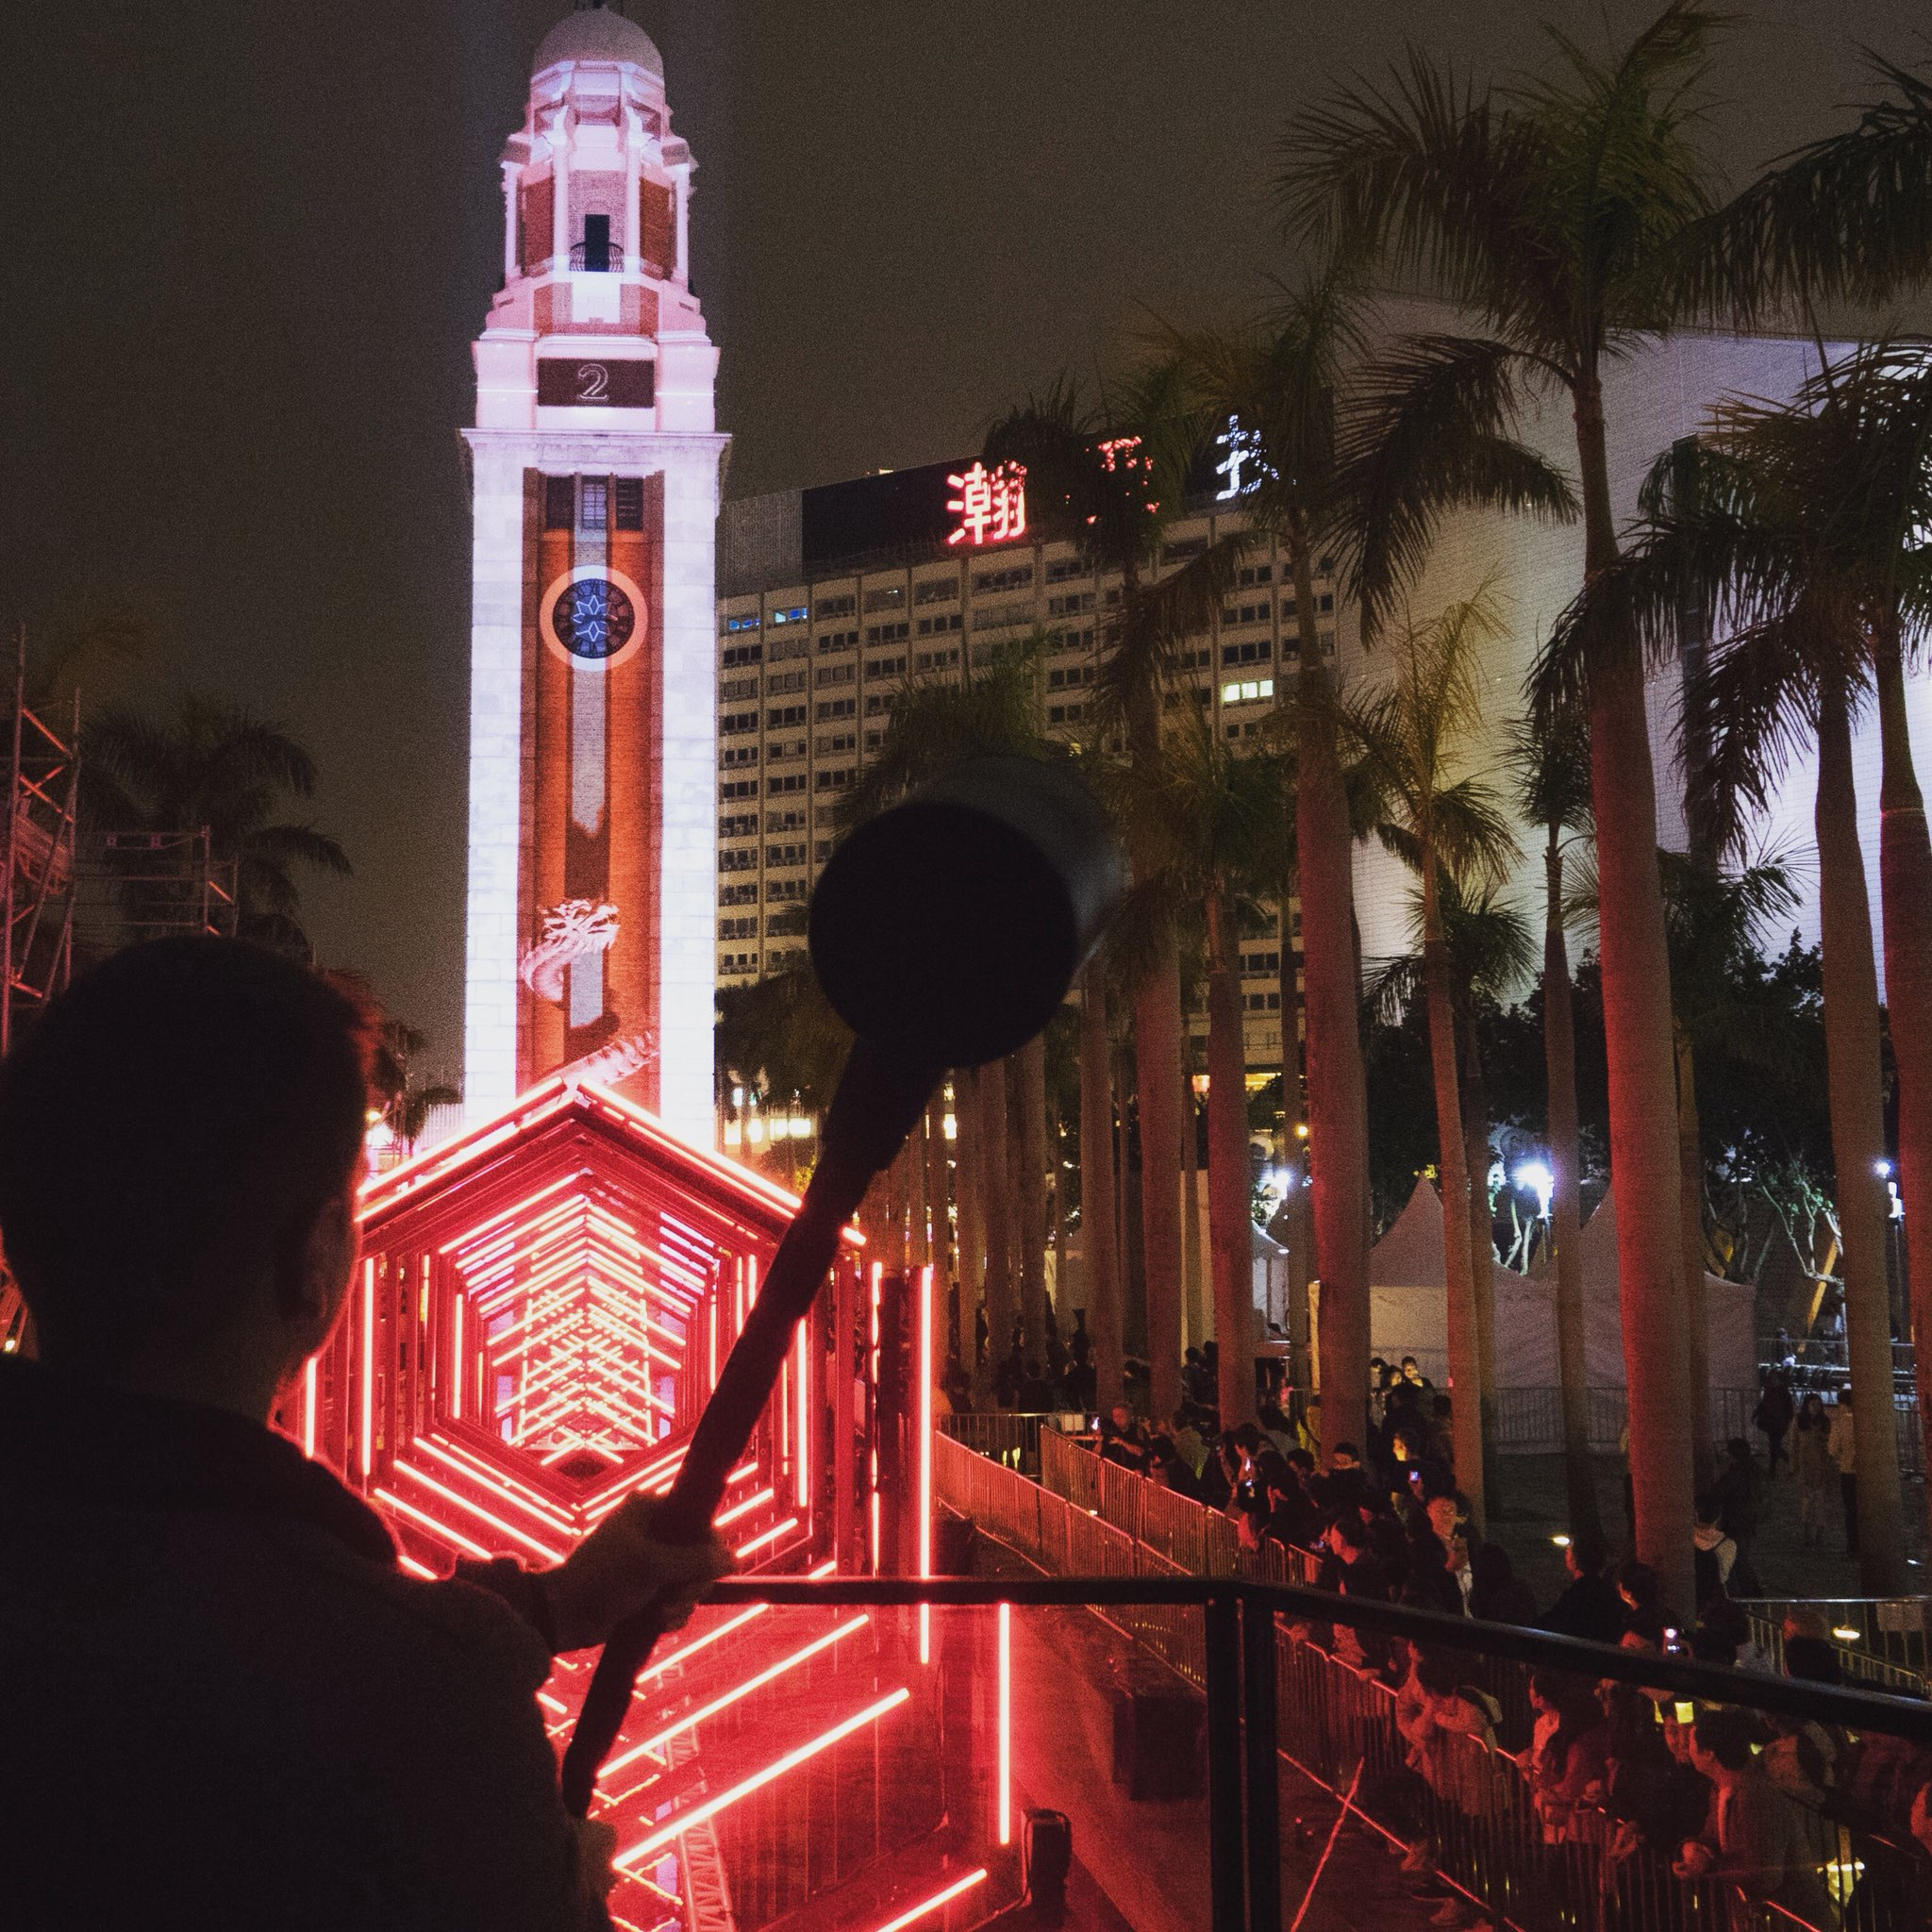
\includegraphics[scale=0.15]{img/long-striker.jpg}
    \caption{L'installation "Long Striker" à la fête des Lumières de Hong Kong}
\end{figure}

\clearpage

\subsubsection{Clients}

Les clients de LTBL et de Vendredi 4 sont, le plus souvent, de la région Rhône-Alpes, mais peuvent aussi être en région parisienne.
Ces clients sont des PME ou des grands groupes désirant de nouvelles installations interactives pour leurs showrooms.
Au travers de ces installations, ils peuvent montrer leur produit de manière esthétique à leurs clients.
Les showrooms ne sont pas les seuls installations organisées par LTBL, on retrouve aussi des présentations de produits pour les salons ou l'affichage de données pour la productivité.

\bigskip

Quelques clients :

\begin{multicols}{2}
    \begin{itemize}
        \item Biomérieux
        \item EDF
        \item Michelin
        \item Somfy
        \item Visiativ
        \item Courchevel
        \item Fête des Lumières
        \item Et bien d'autres \ldots
    \end{itemize}
\end{multicols}

    \subsection{bioMérieux}

BioMérieux est une entreprise spécialisée dans le diagnostic in vitro et dans la microbiologie.
Cette entreprice concoit et fabrique des instruments permettant de diagnostiquer des maladies et de faire des analyses microbiologiques.

BioMérieux dispose d'un showroom permettant de montrer leur produits à leurs futurs clients.
Dans ce Showroom, un ensemble de dispositifs interactifs sont mis en place pour presenter les produits et l'entreprise.
Parmis ces équipement, on retrouve l'espace solution.
Cet espace présente un exemplaire physique des principales machines concus par bioMérieux.
Un projecteur permet alors d'afficher une image sur une vitre opacifiante.
On utilise alors une application pour montrer 

    \section{Blind Test \aha}

\subsection{\ah Arena}

\ah est le premier gérant d'hôtel de France et le 6e mondial.
À l'occasion d'un partenariat, le Palais omnisports de Paris-Bercy s'est vu renommé \aha pour 10 ans.

Le site accueillant beaucoup de concerts et de spectateurs, Accorshotel a voulu communiquer au travers d'une installation interactive.
Cette installation est un blind test composé d'un écran et d'un iPad permettant de saisir les réponses.

Le jeu est simple : une chanson est jouée sur l'écran et le titre de cette chanson est indiqué.
Le joueur dispose alors de 45 secondes pour trouver l'artiste en question parmi les 4 proposé.
On enchaîne ainsi sur 6 questions qui se terminent sur le résultat du jeu affiché à l'utilisateur.

\subsection{Technologies}

Les technologies utilisées dans ce projet sont standards et étaient déjà maîtrisées par les membres de l'équipe.
On retrouve alors une application \emph{Electron} pour l'affichage sur l'écran et un serveur NodeJS avec le framework \emph{Express} pour servir les fichiers et gérer le jeu.
Enfin, on utilise \emph{Socket.io} pour les WebSocket apportant de l'interactivité.

\subsubsection{Express}

Express est une librairie utilisant les capacités de NodeJs (inclus dans \emph{Electron}) à mettre en place un serveur Web.
Express permet de répondre à une URL, mais aussi de servir des fichiers en tout genre.

Nous avons choisi Express car il est léger et simple à mettre en place.
Il dispose d'une grande communauté et permet de mettre en place un serveur Web et websocket rapidement.

Nous n'avions pas besoin ici d'une solution plus lourde car les seules interactions HTTP sont les demandes de médias comme la musique et les images ou la demande de page WEB.
Le reste des interactions s'effectuent au travers des Websockets.

\subsubsection{WebSockets}

La technologie de Websocket est un protocole Web de connexion bidirectionnel.
Ils permettent au serveur et au client de conserver une connexion TCP bidirectionnelle.

Ainsi il est possible au client d'envoyer des paquets arbitraires au serveur, mais aussi au serveur d'envoyer des paquets au client à n'importe quel moment.
Ainsi, il est possible de rendre l'application très interactive et dynamique.

Nous avons utilisé les WebSockets pour toute la communication entre le serveur et les clients (Écran et iPad) avec l'aide de Socket.io.
Cette librairie se place comme une surcouche aux websocket et reprend l'aspect événementiel de Nodejs.
En effet, elle met à disposition du développeur un objet \texttt{socket} agissant comme un émetteur et un récepteur d'événements.
Chaque événement est composé d'un nom et d'un objet de contexte.
Lors de l'émission, l'objet \texttt{socket} transmet l'événement et le contexte au client connecté.
Il est aussi possible de recevoir des événements et ainsi de communiquer de manière bidirectionnelle.

\subsection{Structure}

Le Blind Test se compose de 3 éléments.

\paragraph{Le serveur Web} présent dans le processus principal de l'application Electron, il gère tout le jeu du début à la fin.
Il présente un serveur de fichiers permettant l'accès aux fichiers audio, aux fichiers d'image et aux pages Web depuis l'iPad et l'affichage.
Il dispose aussi d'un serveur WebSockets permettant une communication bidirectionnelle entre les clients (iPad et TV) et le serveur.

Ce serveur Web dispose d'un état définissant l'état actuel du jeu.
Cet état est transmis à tous les clients pour qu'ils actualisent leurs affichages lors d'un changement et de la connexion d'un nouveau client.

Le serveur Web construit en parallèle un objet Javascript \texttt{Game} contenant toutes les questions à poser, la question actuellement posée, les réponses des joueurs et le score.
Cet objet \texttt{Game} est transmis à chaque client lors de leur connexion ou lors du changement d'état du jeu.

Dès que l'état du jeu change, un événement socket.io est transmis à tous les clients connectés pour qu'ils actualisent leur affichage en fonction des données transmises par le serveur.

\paragraph{Les clients (TV et iPad)} Chacun charge une page HTML spécifique possédant un script spécifique.
Ce script va afficher le bon écran en fonction de l'état du jeu envoyé par le serveur et, éventuellement, demander une interaction à l'utilisateur.

Dès qu'un joueur tape sur une réponse, l'iPad envoie à son tour un paquet WebSocket au serveur pour qu'il l'enregistre et change d'état.
Le jeu continue alors jusqu'à ce que toutes les questions de tous les joueurs soient posées.

\begin{figure}[h]
    \centering
    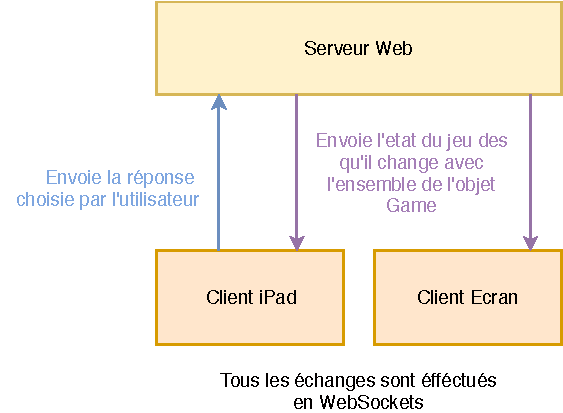
\includegraphics{img/ah-blindtest.pdf}
    \caption{Structure du jeu Blind Test}
\end{figure}

\subparagraph{TV} Coté TV, l'affichage est simple et permet d'afficher le score de l'utilisateur ainsi que de jouer la musique.
L'écran n'étant pas tactile, il ne permet que l'affichage d'informations sur l'état du jeu, mais aucune interactivité n'est possible directement.
Le client TV est une fenêtre de l'application Electron qui se connecte au serveur express pour charger l'interface.

\subparagraph{iPad} Coté iPad, une application de kiosque permet d'afficher une page Web sans autre élément d'interface.
Cette page Web est chargée depuis le serveur et propose des choix à l'utilisateur en fonction de l'état du jeu.
Cela peut être le nombre de joueurs, le nom de l'artiste en cours de lecture ou simplement une demande pour passer à la question suivante.

\subsubsection{Design}

Le design de l'application était fourni avec la demande du client et nous avons juste intégré ce design en extrayant des images clés du fichier Photoshop du designer.

\begin{figure}[h]
    \centering
    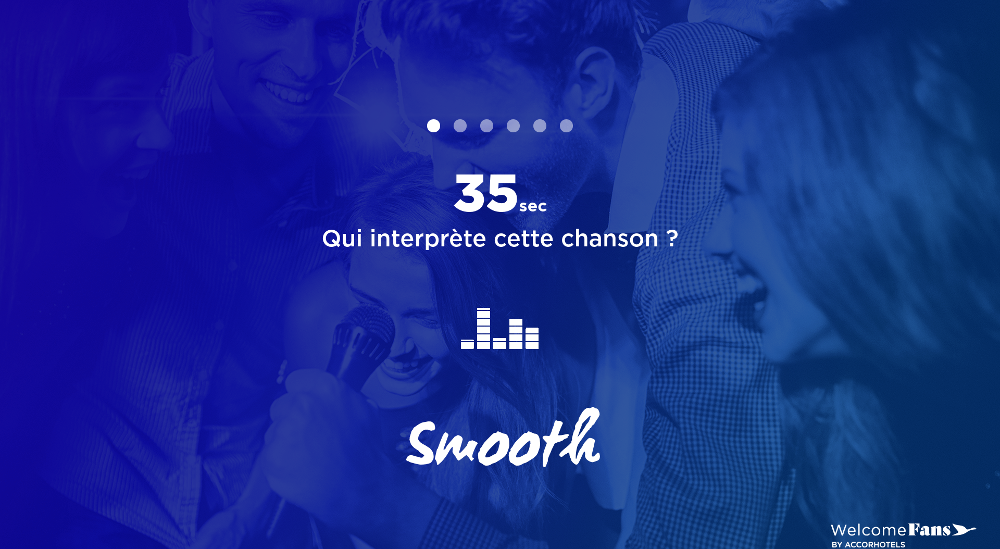
\includegraphics[scale=0.23]{img/blind-test-tv.png}
    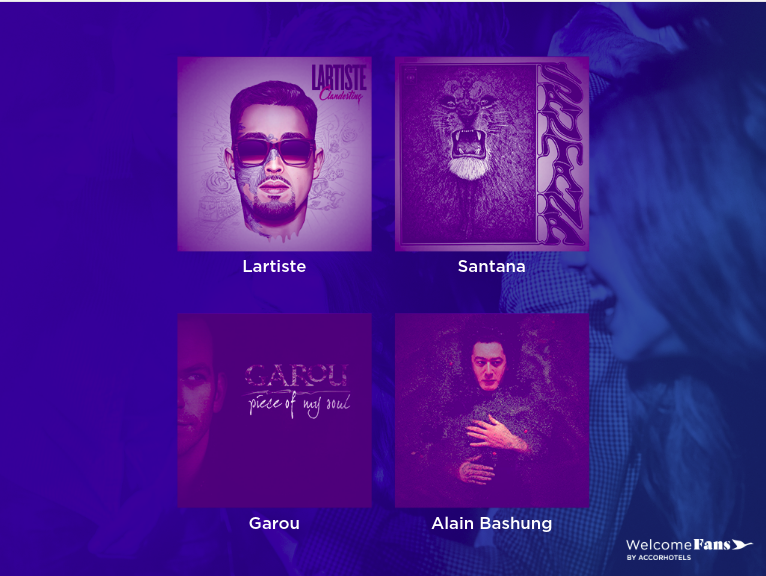
\includegraphics[scale=0.22]{img/blind-test-ipad.png}
    \caption{Une vue du Blind Test côté TV (à gauche) et côté iPad (à droite)}
\end{figure}

\subsubsection{Installation}

Je n'ai pas pu assister à l'installation du lundi 29 janvier, mais j'ai tout de même travaillé dessus à l'occasion de correction de bugs.

L'installation présente un grand écran connecté au serveur affichant l'interface TV sur une machine Windows hébergeant le serveur websocket que l'iPad pourra contacter.
On y retrouve bien évidemment L'iPad verrouillé pour éviter de sortir de l'application.
Ces deux terminaux sont connectés à une même borne WiFi permettant de disposer de son propre réseau évitant ainsi les latences dues à une éventuelle surcharge du réseau environnant.
Cette borne WiFi fait office de routeur vers l'extérieur, mais aussi de serveur DHCP et de point d'accès WiFi.

\begin{figure}[h]
    \centering
    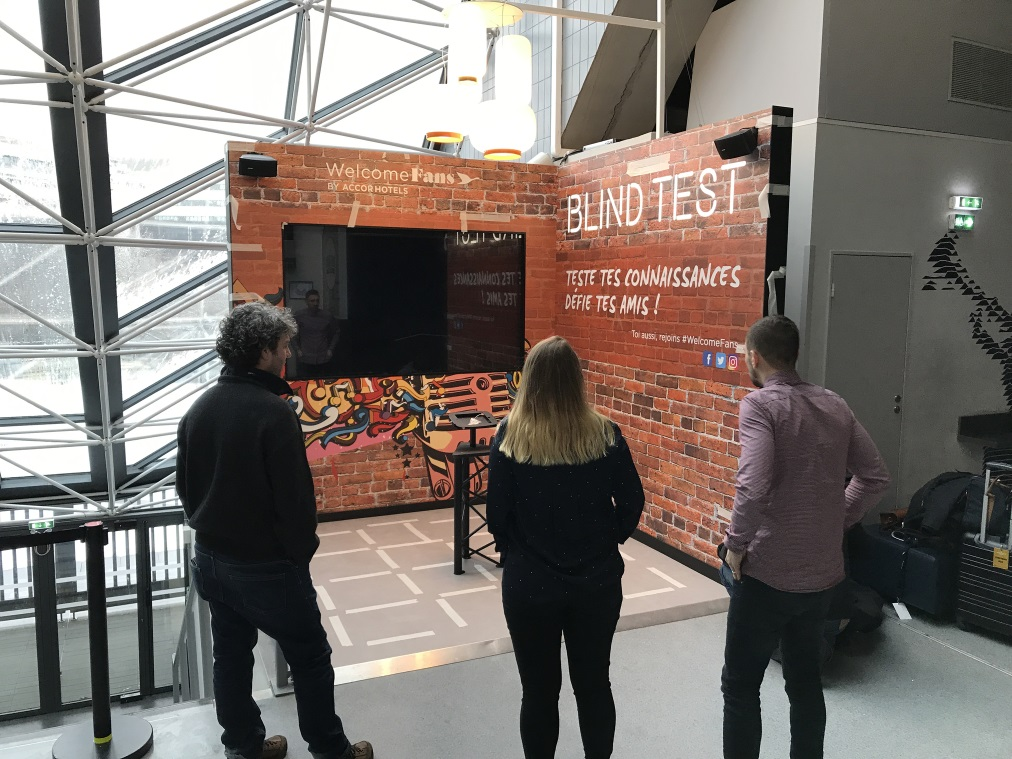
\includegraphics[scale=0.4]{img/accorhotel-blindtest-resize.jpg}
    \caption{Installation du Blind test au \aha}
\end{figure}

\subsubsection{Conclusion}

Ce projet fut intéressant et intense, car nous l'avons réalisé en seulement 2 jours.
Ce fut une bonne expérience de travail d'équipe et m'a permis de tester un projet à court délai.
Enfin, ce projet m'a permis de voir les techniques permettant de synchroniser l'état de multiples machines au travers de Websocket.


    \section{Bornes de présentation Somfy}

\subsection{Somfy}

Somfy est un entreprise concevant des systèmes domotiques à l'attention du grand public.
Dans une démarche de communication, Somfy a contacté LTBL pour la creation de 11 bornes interactives qui seront mises en place dans les magasins vendant les produits de la marque.

\subsection{Besoins}

L'objectif de ce projet est de concevoir et de produire 11 machines permettant d'afficher des informations sur l'entreprise et ses produits.
Ces informations peuvent être des vidéos, du texte ou des images.

Dans ce projet, je n'ai pas travaillé sur le développement de l'application de présentation mais sur la mise en place des 11 machines permettant son execution.
Ces 11 machines devaient presenter un système de visionnage pour réduire au maximum les possibilités de l'utilisateur.

\subsection{Recherches et choix du système}

Pour ce nouveau projet, j'ai proposé à mon maître de stage d'utiliser un système Linux pour l'execution des applications sur les bornes.
Cela a pour avantage une plus grande flexibilité et capacité de customisation mais aussi une gratuité de la license.
En effet, il est simple de mettre en place un système captif sur une machine linux car on contrôle chaque élément de l'OS .

Pour le système je me suis dirigé vers un membre de la famille Ubuntu pour sa stabilité et la grande communauté qui se forme autour.

J'ai alors découvert Ubuntu Core qui permet la creation de système embarqués et minimalistes.
Ubuntu Core est une varante de Ubuntu se basant sur des paquets unitaire séparés les uns des autres.
Cela permet de séparer chaque application et d'autoriser leur communication sur certains canaux particulier appelés interfaces.
Ce système rapelle beaucoup les systèmes mobiles comme Android ou IOS exigeant des permissions définies à l'avance pour que les applications aient acces à certaines fonctionnalités.
Ubuntu Core utilise Snapcraft, un gestionnaire de paquet permettant cette séparation des applications.
De pars sa complexitée et de l'abscense de serveur X sur snapcraft, je n'ai pas retenu cette solution et me suis penché sur Ubuntu Server.

Ubuntu Server est une version de Ubuntu sans les composants de bureau classique.
Il permet de composer son propre système sans la lourdeur des applications graphiques inutiles dans le contexte des bornes Somfy.
J'ai donc choisi cette distribution ayant pour objectif d'installer un environnement de bureau manuellement.

\subsection{Environnement de kiosk}

Pour mettre en place l'environnement d'affichage, j'ai commencé par installer le serveur X .
Le serveur X est le logiciel en charge d'afficher l'interface à l'utilisateur au travers d'un protocol spécifique.

Apres avoir installé ce logiciel, il faut installer un système de gestion de fenètres qui sera en charge d'afficher les différentes fenêtre à la bonne taille et dans le bon contexte.
Pour le gestionnaire de fenêtres, j'ai choisi xfce car il est légé et propose beaucoup de fonctionnalités.
Le gestionnaire de fenêtre est essentiel car il permet aux applications de correctement se dimentionner et de passer en plein ecran pour empècher l'utilisateur d'éfféctuer des actions non désirées.

Enfin, on peut installer notre application et la démarrer.

Il faut bien sur automatiser tout cela pour que l'ensemble puisse se démarrer automatiquement en même temps que la machine pour éviter tout action manuelle de l'installateur.
Pour ce faire j'ai été amené a modifier le pipeline de démarrage du système.
Tout d'abord il faut créer un nouvel utilisateur qui sera en charge d'executer l'application pour eviter qu'elle ne soit éxécuté en tant qu'administrateur.
Ensuite, il faut modifier le comportement de connexion sur la première console pour qu'elle se connecte automatiquement avec l'utilisateur en charge de l'execution du programme.
L'utilisateur connecté, on execute le script de démarrage qui se charge de démarrer le serveur X, le gestionnaire de fenêtres et l'application.

Nous disposons alors d'un système de kiosk fonctionnel et sécurisé.

\subsection{Système de mise à jour}

Pour permettre un mise à jour de l'application simplifiée j'ai été amené à réfléchir sur un système de mise à jour.
Il n'est pas possible de connecter la borne à internet et cela implique que l'on ne peut pas mettre à jour à distance.
Il fallait donc trouver un solution permettant de changer les fichiers de l'application sans pour autant nécéssiter la rapatriement des bornes chez LTBL .

Pour ce système j'ai choisi d'utiliser un ensemble de scripts bash permettant d'avoir un grand contrôle sur le système avec un système de scripting simple et rapide.

Le système de mise à jour que j'ai mise en place se compose de 3 elements clés

\paragraph{Watching USB} Linux dispose d'un système de gestion des périphériques appelé \texttt{udev}.
Ce système permet de gerer le connexion, la déconnexion et le montage des elements amovibles du système.
En ajoutant des rêgles dans le fichier de configuration spécifique de udev, on peut executer une commande lors de la connexion ou la déconnexion d'un périphérique amovible.
J'ai utilisé cette fonctionnélité pour vérifier si le support contien une mise à jour et lancer l'installation de la mise à jour dans ce cas.

\paragraph{Fichier de verrouillage} Lors d'une mise à jour, le script installant cette mise àjour créer un fichier \texttt{update.lock} à la racine de l'application permettant d'indiquer que'une mise à jour est en cours.
Il arrete alors de force l'application en cours d'éxécution pour l'installation de la mise à jour.
On ajoutera alors au fichier \texttt{update.lock} les logs de toute la mise à jour pour suivre en temps reel sont déroulement.

\paragraph{Scripts de mise à jour} Pour éviter que l'on puisse executer du code arbitraire en tant qu'administrateur sur la machine, seul un nombre limité d'actions peuvent être éfféctués durant une mise à jour.
Chaque action représente un script dans le dossier \texttt{update} à la racine de l'application.
Chacune de ces actions disposent de ses paramètres.

\medskip

Chque mise à jour de l'application passe donc par un support amovible ce qui permet à n'importe quel personne de l'efféctuer.
Ce support amovible contien un fichier \texttt{update.conf}, un fichier texte décrivant pas à pas la procedure à adopter.
Seul les actions disponibles sur la machine peuvent être éxécutés, la procedure n'est donc pas composée de commandes bash mais de noms de scripts présents dans le fichier \texttt{update}.
Chaque mise à jour est aussi asosciée à un numéro de version présent dans le fichier \texttt{update.version}.
Ce fichier est vérifié et sera copié à la fin de la mise à jour à la racine de l'application pour ne pas faire deux fois les mêmes opérations.

%TODO donner un exemple de conf

\subsection{Materiel \& Installation}

Les machines en charge d'héberger l'appliction sont des NUC d'intel.
Les NUC sont des mini machines crées par Intel et disposant d'un processeur directement soudé sur la carte mêre.
Ces machines on l'avantage d'être trés compact.

\begin{figure}[h]
    \centering
    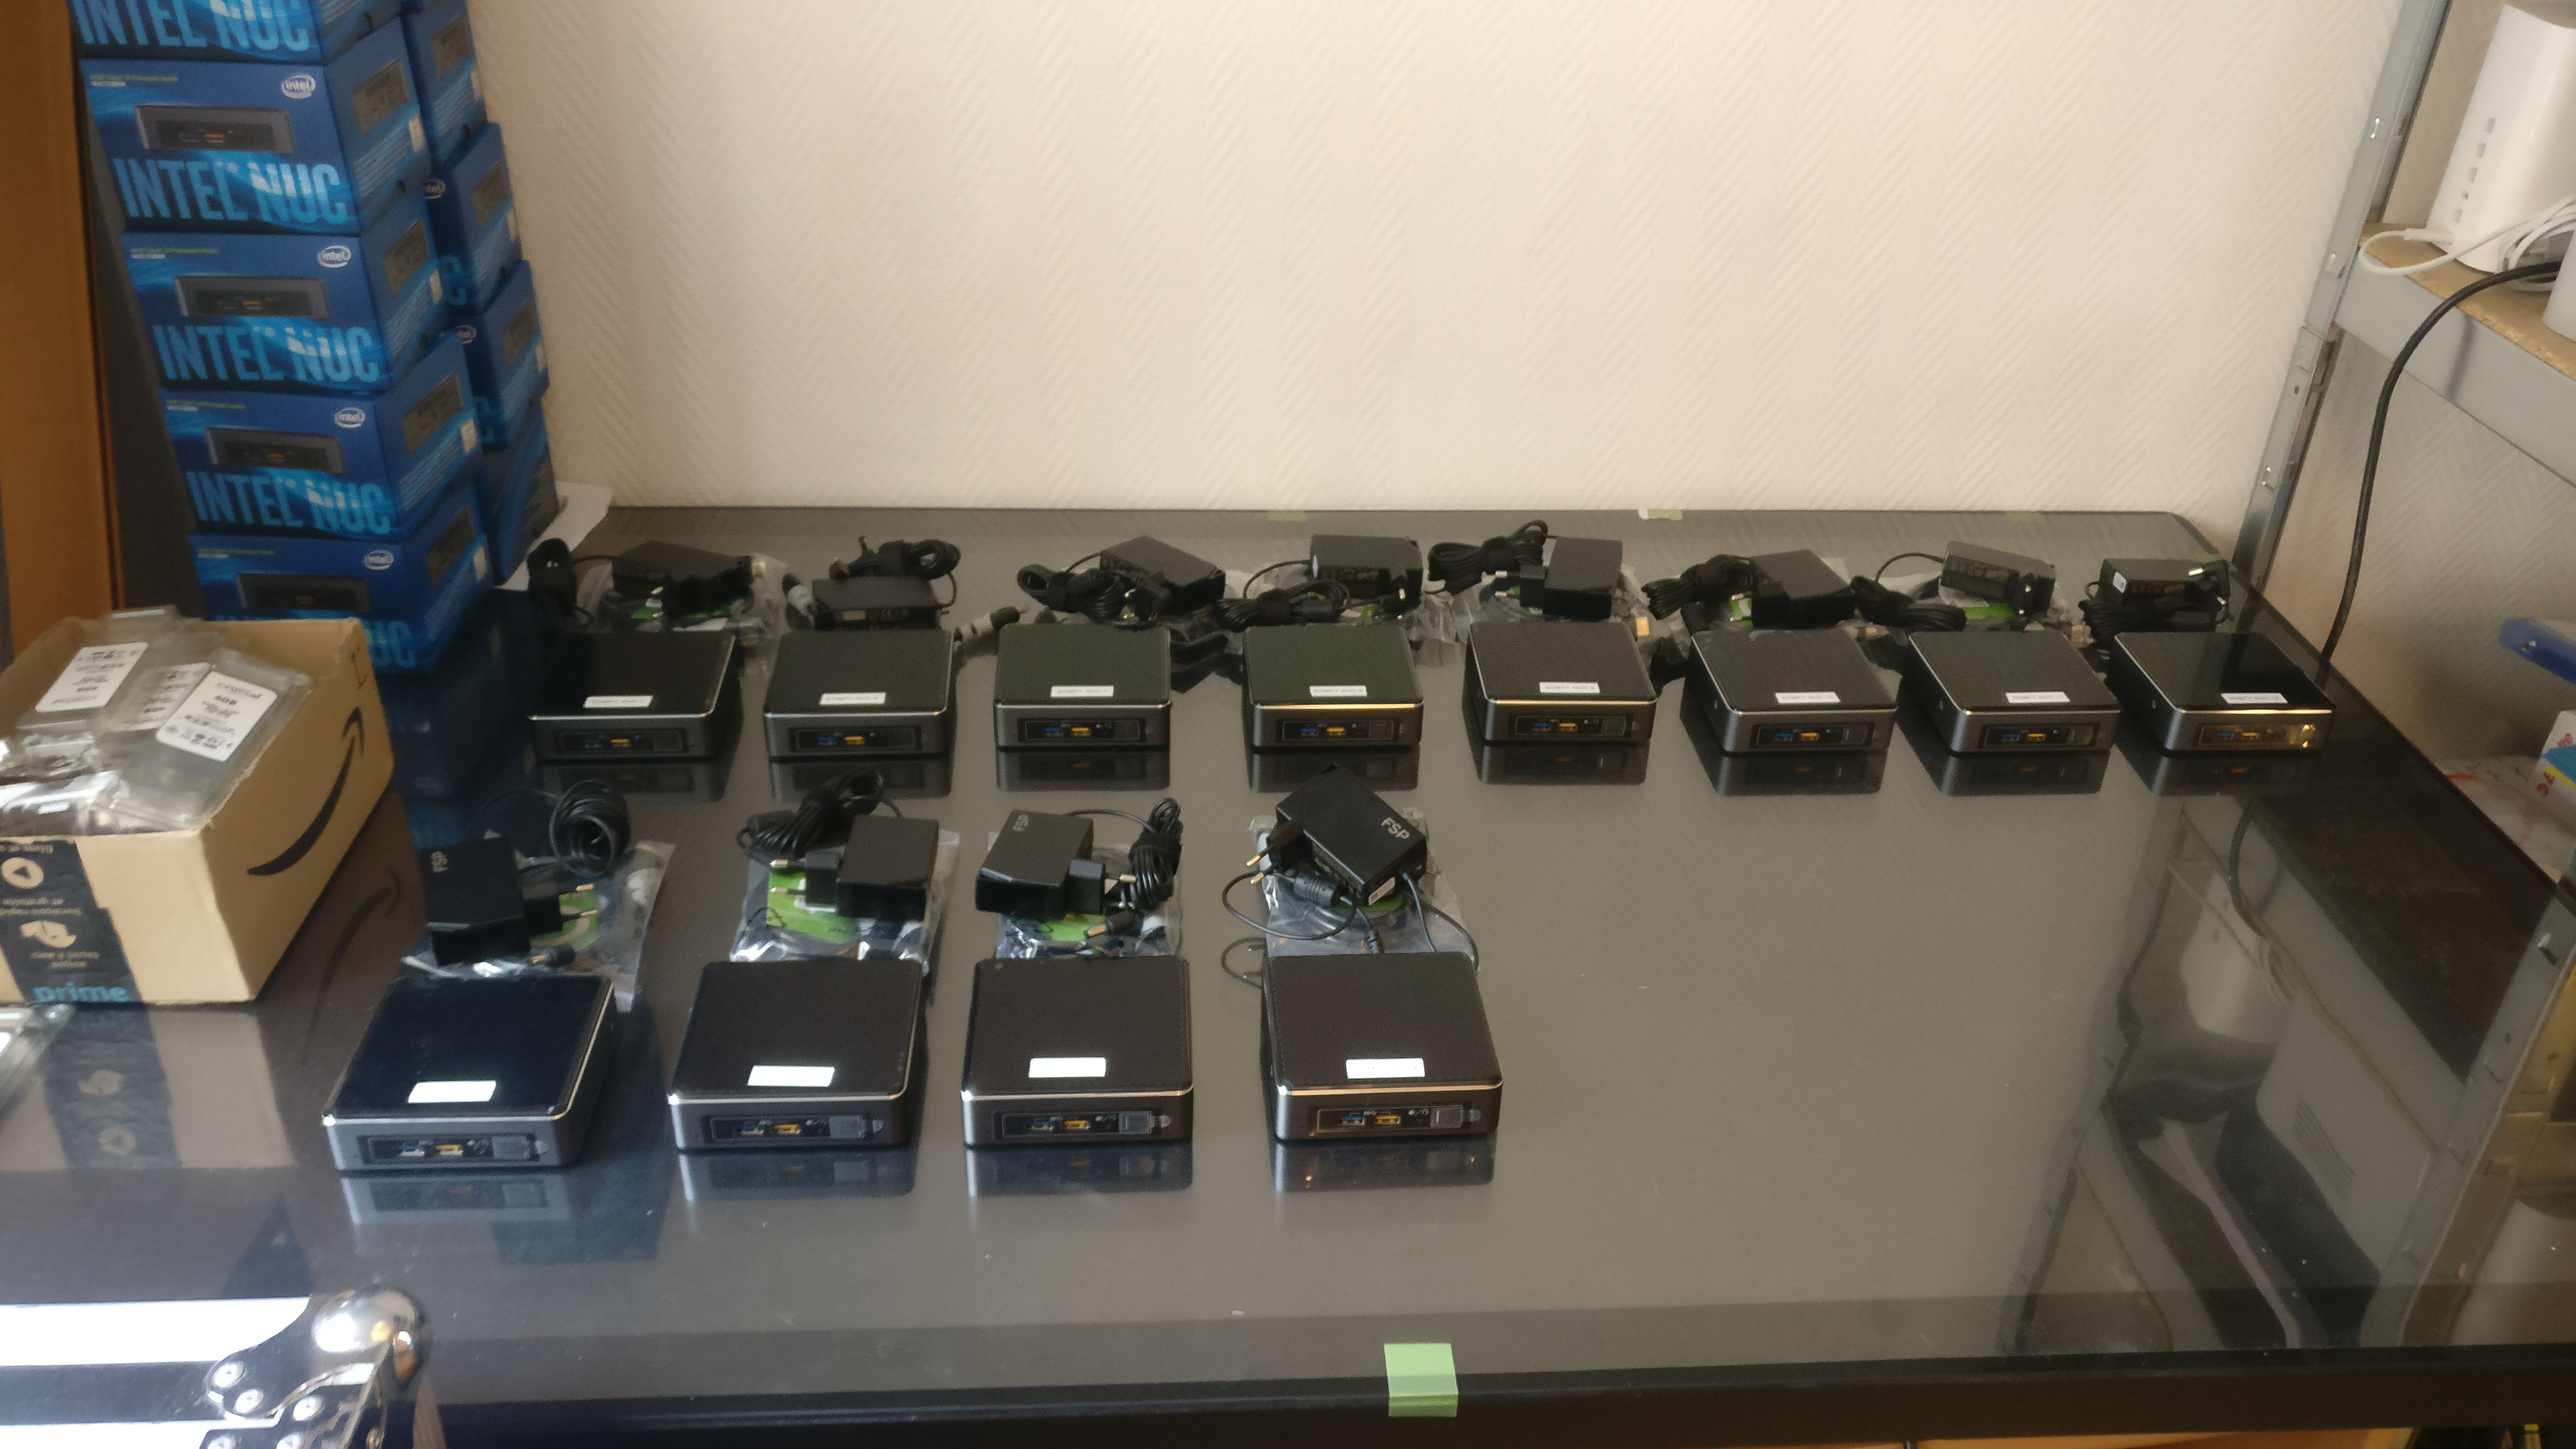
\includegraphics[scale=0.1]{img/somfy-nuc.jpg}
    \caption{Les 12 NUC hebergeant l'application de présentation}
\end{figure}

J'ai donc installé le système sur une machine que l'on apellera master.
J'ai ensuite utilisé CloneZilla pour faire une image du disque de cette machine et pouvoir la répliquer.

Apres l'installation, nous avons trouvé quelques problèmes qui devaient être corrigés.
N'ayant pas le temps de réinstaller un clone sur toutes les machines, nous avons mis en réseau toutes les machines.
Il suffit alors d'utiliser \texttt{cssh} pour éfféctuer les mêmes actions en sychronisé sur toutes les machines.
\texttt{cssh} est un utilitaire permettant de créer un certain nombre de terminaux ssh tous synchronisés;
Il est alors aisé d'administrer un ensemble de machines en même temps.

\begin{figure}[h]
    \centering
    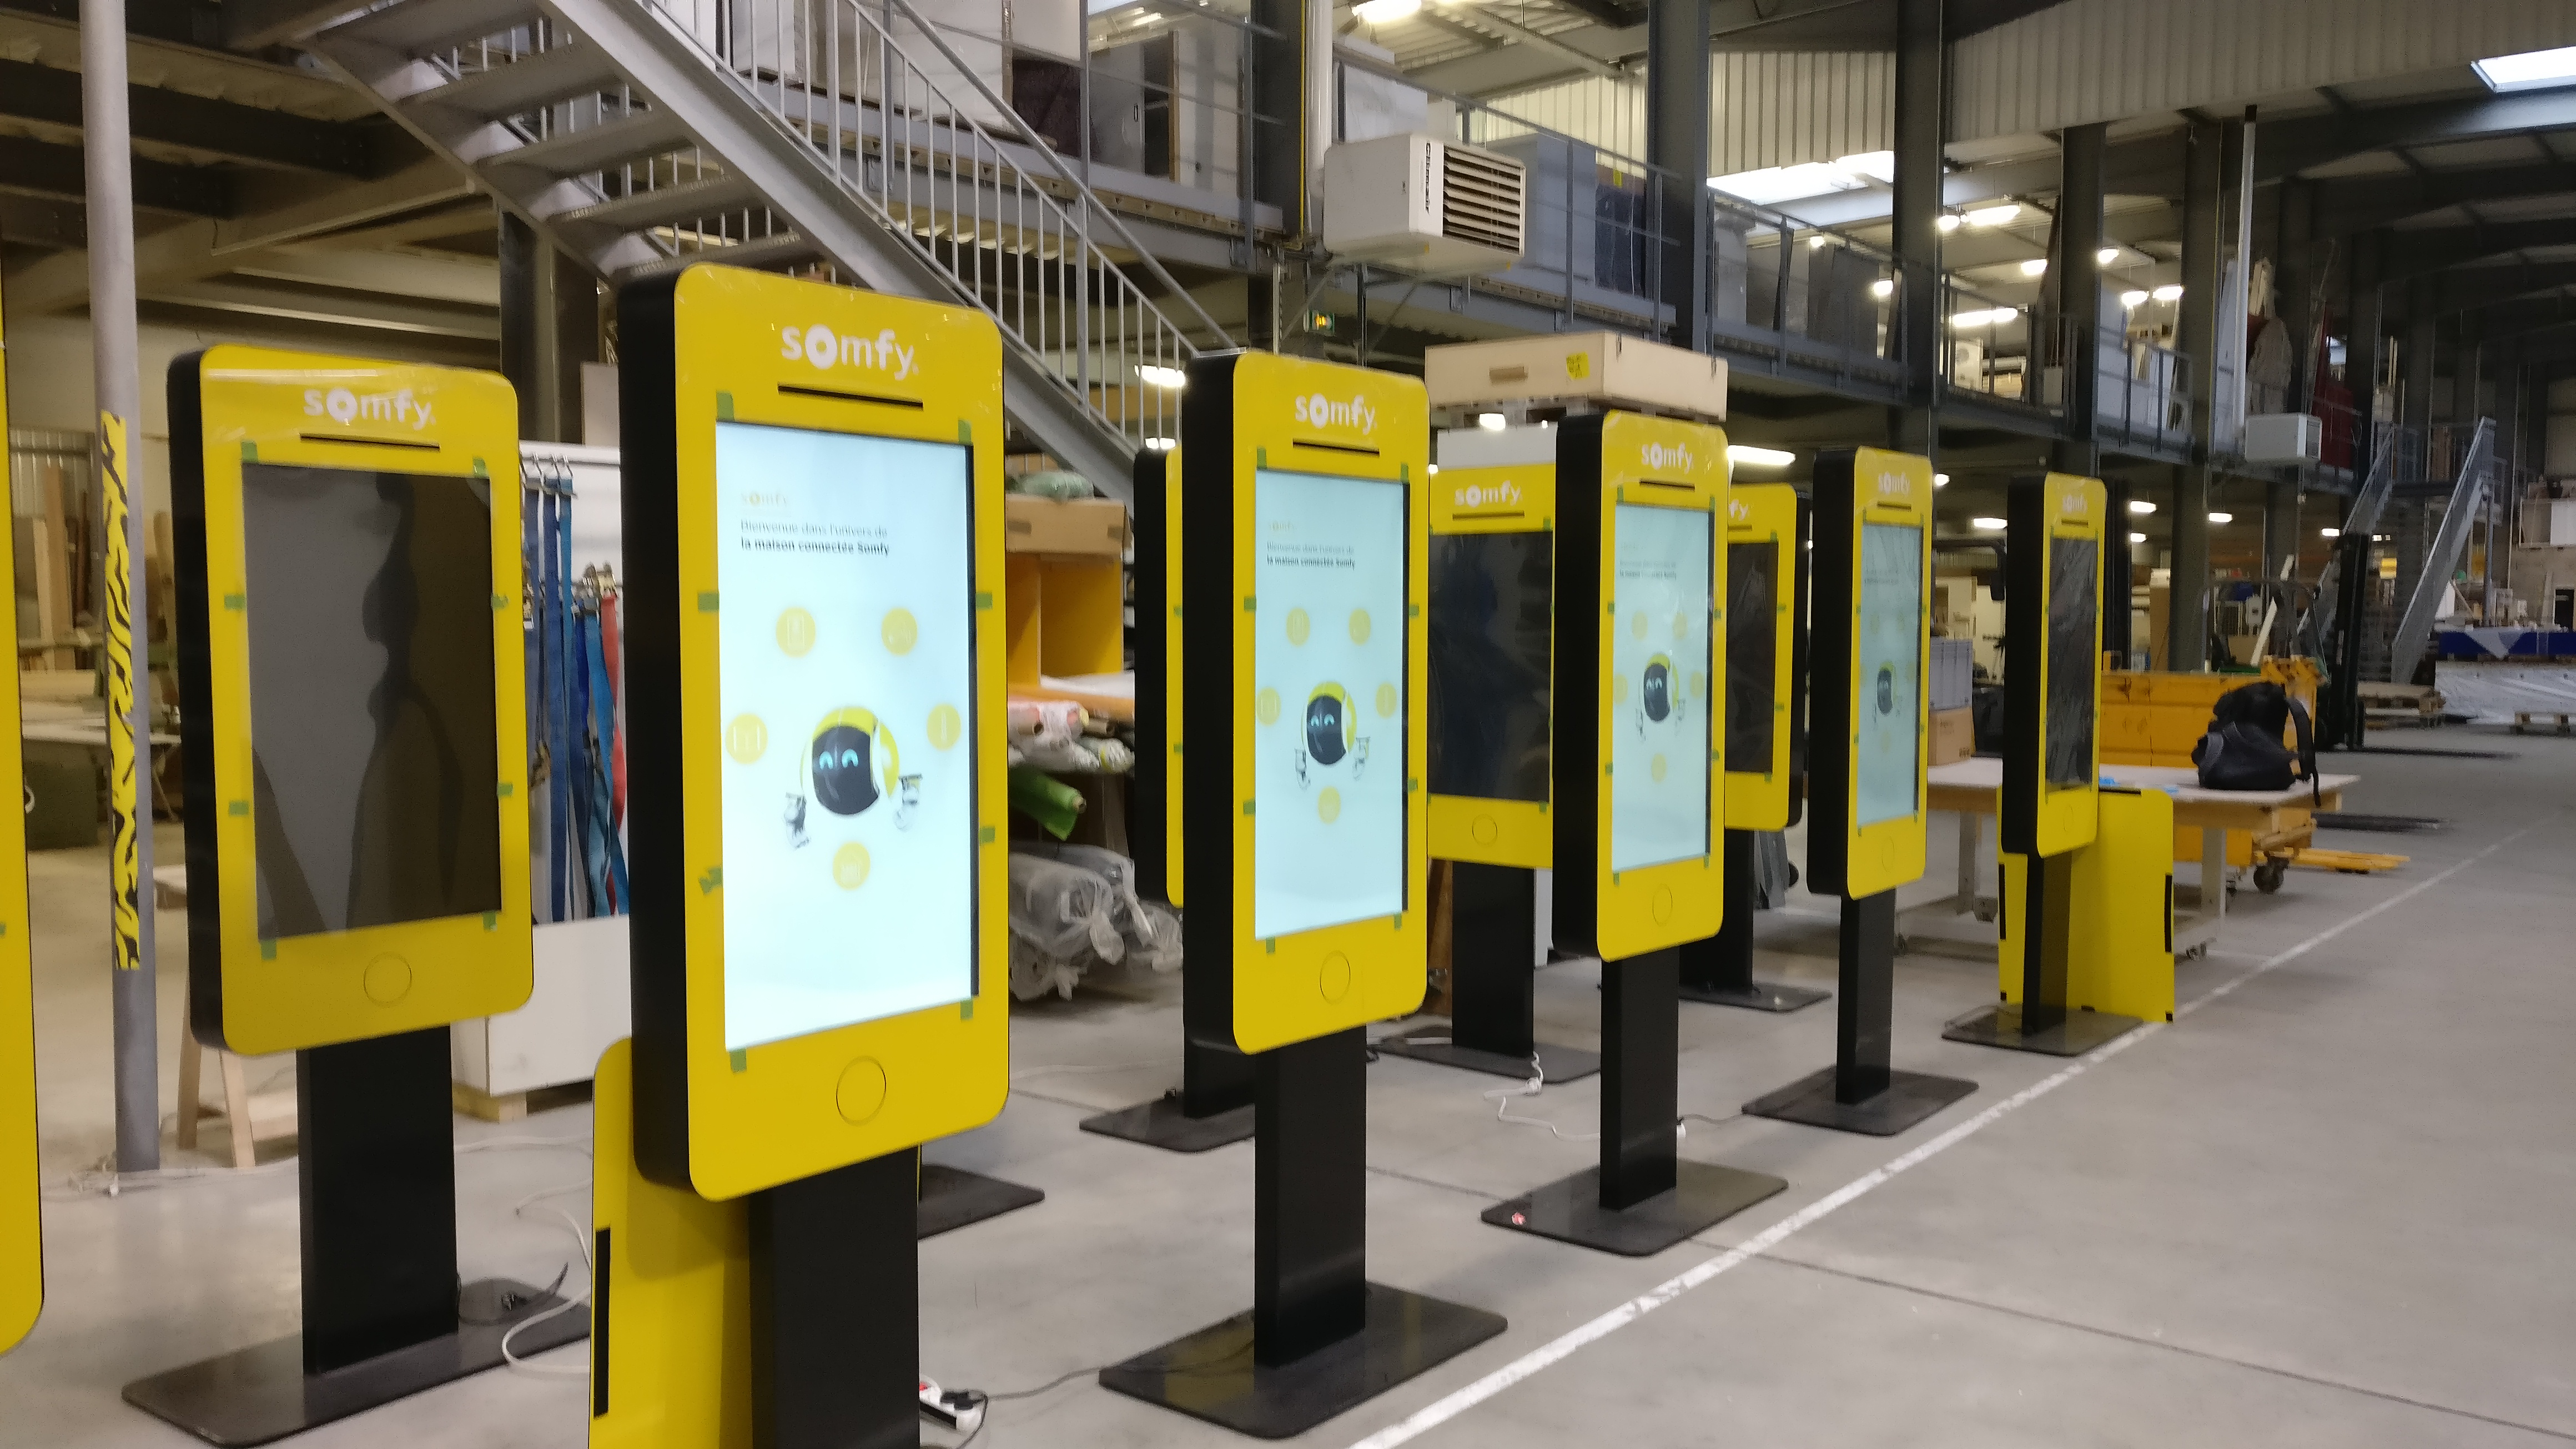
\includegraphics[scale=0.1]{img/somfy-install.jpg}
    \caption{Bornes Somfy lors de l'installation des machines dans leurs abitacles}
\end{figure}

\subsection{Conclusion}

Ce projet fut interessant car il m'a permis de me plonger plus en profondeur sur les composants d'un système linux pour controler son focntionnement.
Malgré la grande partie de recherche pour dégager la meilleur solution, j'ai quand mee eu l'occasion de travailler surn un système de mise à jour innovant.
Le projet est à présent terminé et les bornes ont été disposés dans les magasins vendant la technologie Somfy.

    \section{Media Reader Eiffage}

\begin{figure}[h]
    \centering
    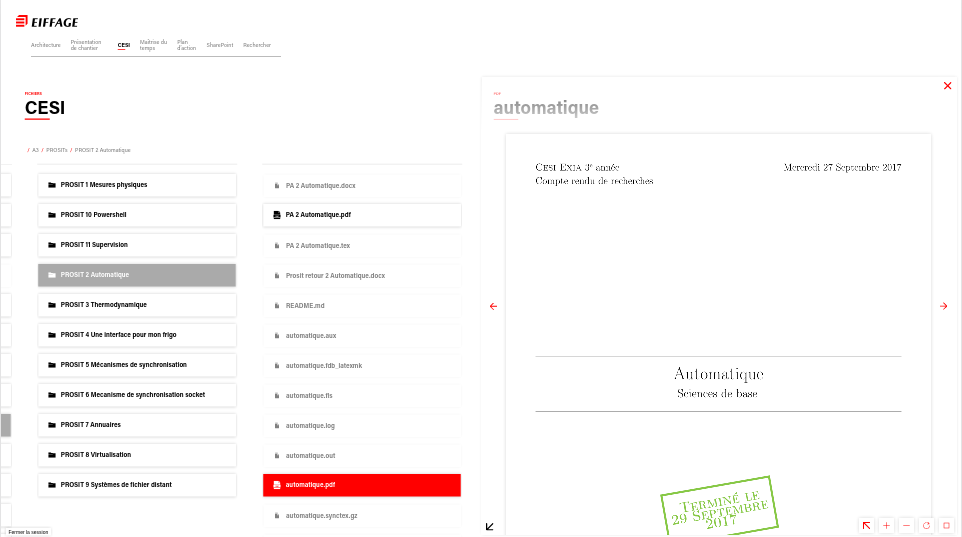
\includegraphics[scale=0.5]{img/media-reader.png}
    \caption{L'interface principale de l'application de lecture des médias Eiffage}
\end{figure}

\subsection{Eiffage}

Eiffage est un grand groupe de traveaux public.
3\up{e} de France, il travaille sur de grands projets dans toute la France.

Dans le cadre de leur chantier de rénovation Laborde, l'objectif était de concevoir une salle de contrôle du chantier connectée.

La salle de contrôle du chantier (appelée salle cockpit) et une salle de réunion des personnes impliquées dans le déroulement du projet de rénovation.
Les plans, les problèmes et les solutions y sont discutés durant toute la durée du projet.
Les plans étudiés sont stockés sur un serveur central et sont disponibles aux employés pour les étudier, les annoter et les commenter.

\medskip

Nous avons mis en place trois solutions pour ce chantier :

La première est une table tactile sur laquelle il est possible d'ouvrir, de manipuler et d'annoter les plans depuis le serveur central.
Cela vient remplacer les impressions successives de plans pour les annotations et les modifications.
Cela permet de réduire la consommation d'encre et de papier mais aussi de gagner du temps.

La seconde est un écran d'affichage permettant de positionner des Post-its sur un plan.
Ces Post-its sont associés à une personne et définissent les tâches à accomplir.

La dernière solution est un explorateur de fichier permettant d'afficher des photos, vidéos ou documents du chantier.
Cette solution a pour objectif de permettre une meilleure présentation du chantier avec des documents directement importés depuis le serveur central.

\medskip

Dans ce projet, j'ai notamment travaillé sur le navigateur de fichier.
Ce navigateur de fichier est affiché sur un écran de 84 pouces tactile mettant à disposition des employés un formidable outil de présentation.

\begin{figure}[h]
    \centering
    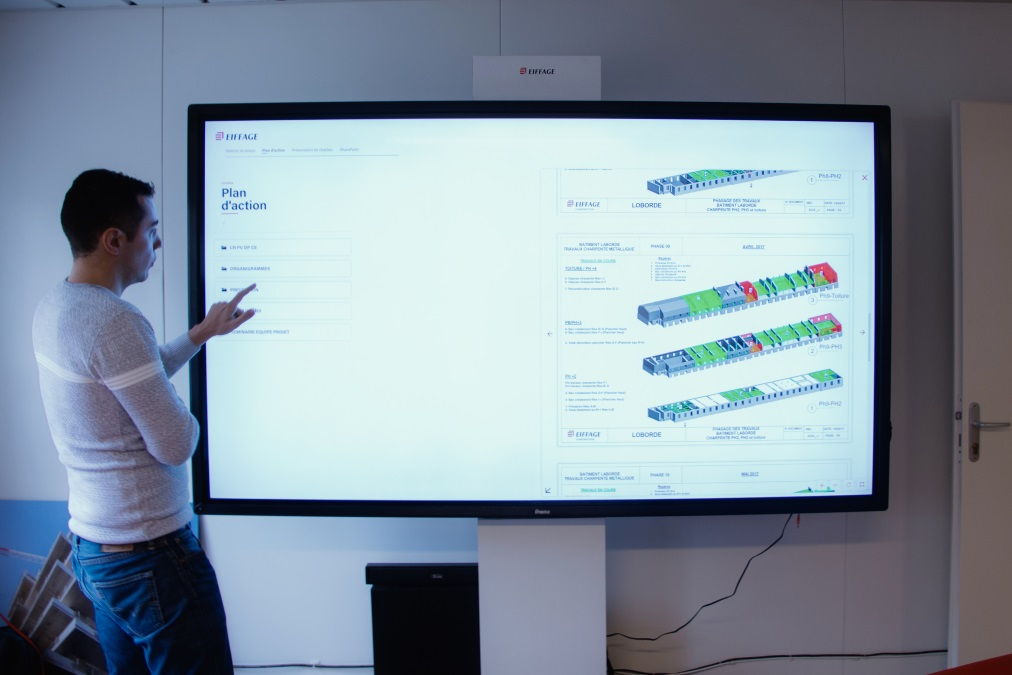
\includegraphics[scale=1.2]{img/media-reader-pres-1.jpg}

    \bigskip

    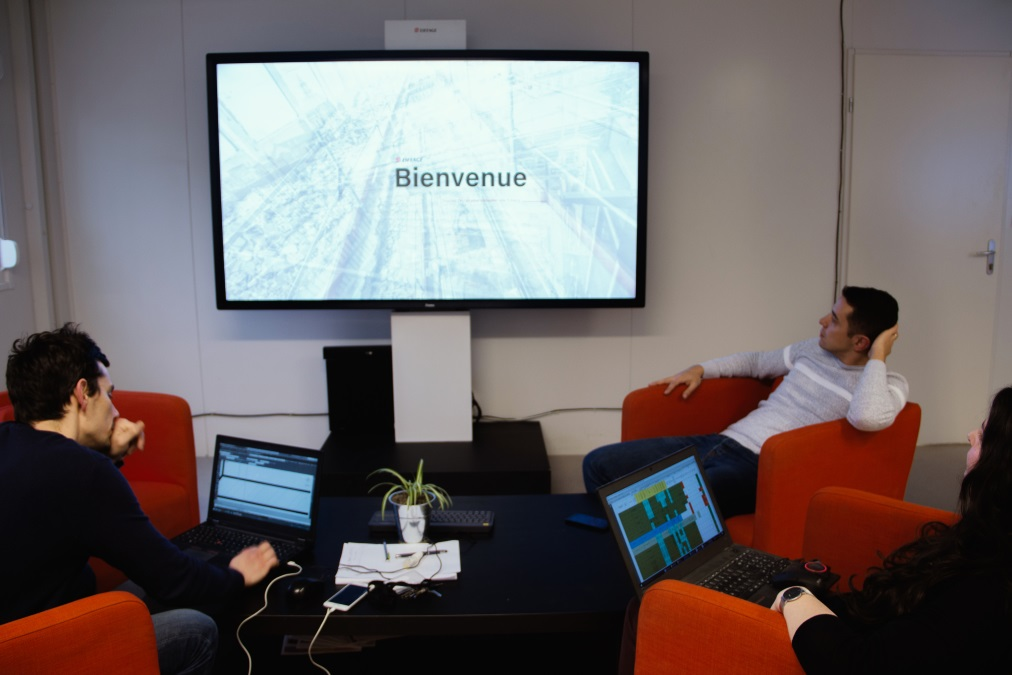
\includegraphics[scale=1.2]{img/media-reader-pres-2.jpg}
    \caption{Un aperçu de l'explorateur de fichier une fois installé dans la salle cockpit}
\end{figure}

\clearpage

\subsection{Lecteur de médias}

Le lecteur de Media Eiffage doit donc disposer des fonctionnalités suivantes :

\begin{itemize}
    \item Se connecter à un emplacement réseau
    \item Lister le contenu des dossiers et pouvoir naviguer dans l'arborescence
    \item Afficher un aperçu des fichier images, vidéo et PDF
    \item Intégrer l'application dans un contexte Active Directory où chaque utilisateur doit pouvoir ouvrir sa session personnelle
    \item Afficher un site internet prédéfini
\end{itemize}

La courte liste des fonctionnalités m'a permis de travailler plus en profondeur sur la structure de l'application et ainsi de développer des fonctionnalités solides.

\subsection{Application existante}

Dû à des retards sur la livraison du matériel requis pour développer les applications Eiffage, le développement était peu avancé.
L'explorateur de fichier chargeait toute l'arborescence de la source des données ce qui était peu optimisé.
En revanche la solution initiale contenant un navigateur de PDF que j'ai repris dans ma version de l'application.

Globalement, j'ai repris une grande partie de l'application qui n'utilisait pas les WebComponents pour l'adapter aux nouvelles techniques Web permettant de modulariser chaque élément de l'interface.

\subsection{Technologies utilisées}

Pour cette application, j'ai décidé d'utiliser la même technologie que les autres applications de LTBL soit Electron et l'utilisation des WebComponents.

Je n'ai pas utilisé de technologie supplémentaire ni de librairie complémentaire pour me former sur les futures normes Web.

\subsection{Structure}

Avec ce projet, j'ai continué à expérimenter avec les WebComponents pour trouver le bon paradigme d'utilisation.
En effet, les WebComponents présentent une structure d'application très différente des applications Web standard.
Chaque composant étant isolé des autres il faut utiliser des systèmes de communication comme les événements JavaScript pour permettre une communication entre les components.

Pour ce projet, j'ai fragmenté mon code sur de multiples niveaux de WebComponents.
Contrairement à l'application de BioMérieux où j'ai fait de grands composants par grande partie de l'application.
Dans cette application, j'ai modularisé au maximum les éléments de l'interface pour pouvoir réutiliser ces composants dans un autre contexte.

\begin{figure}[h]
    \centering
    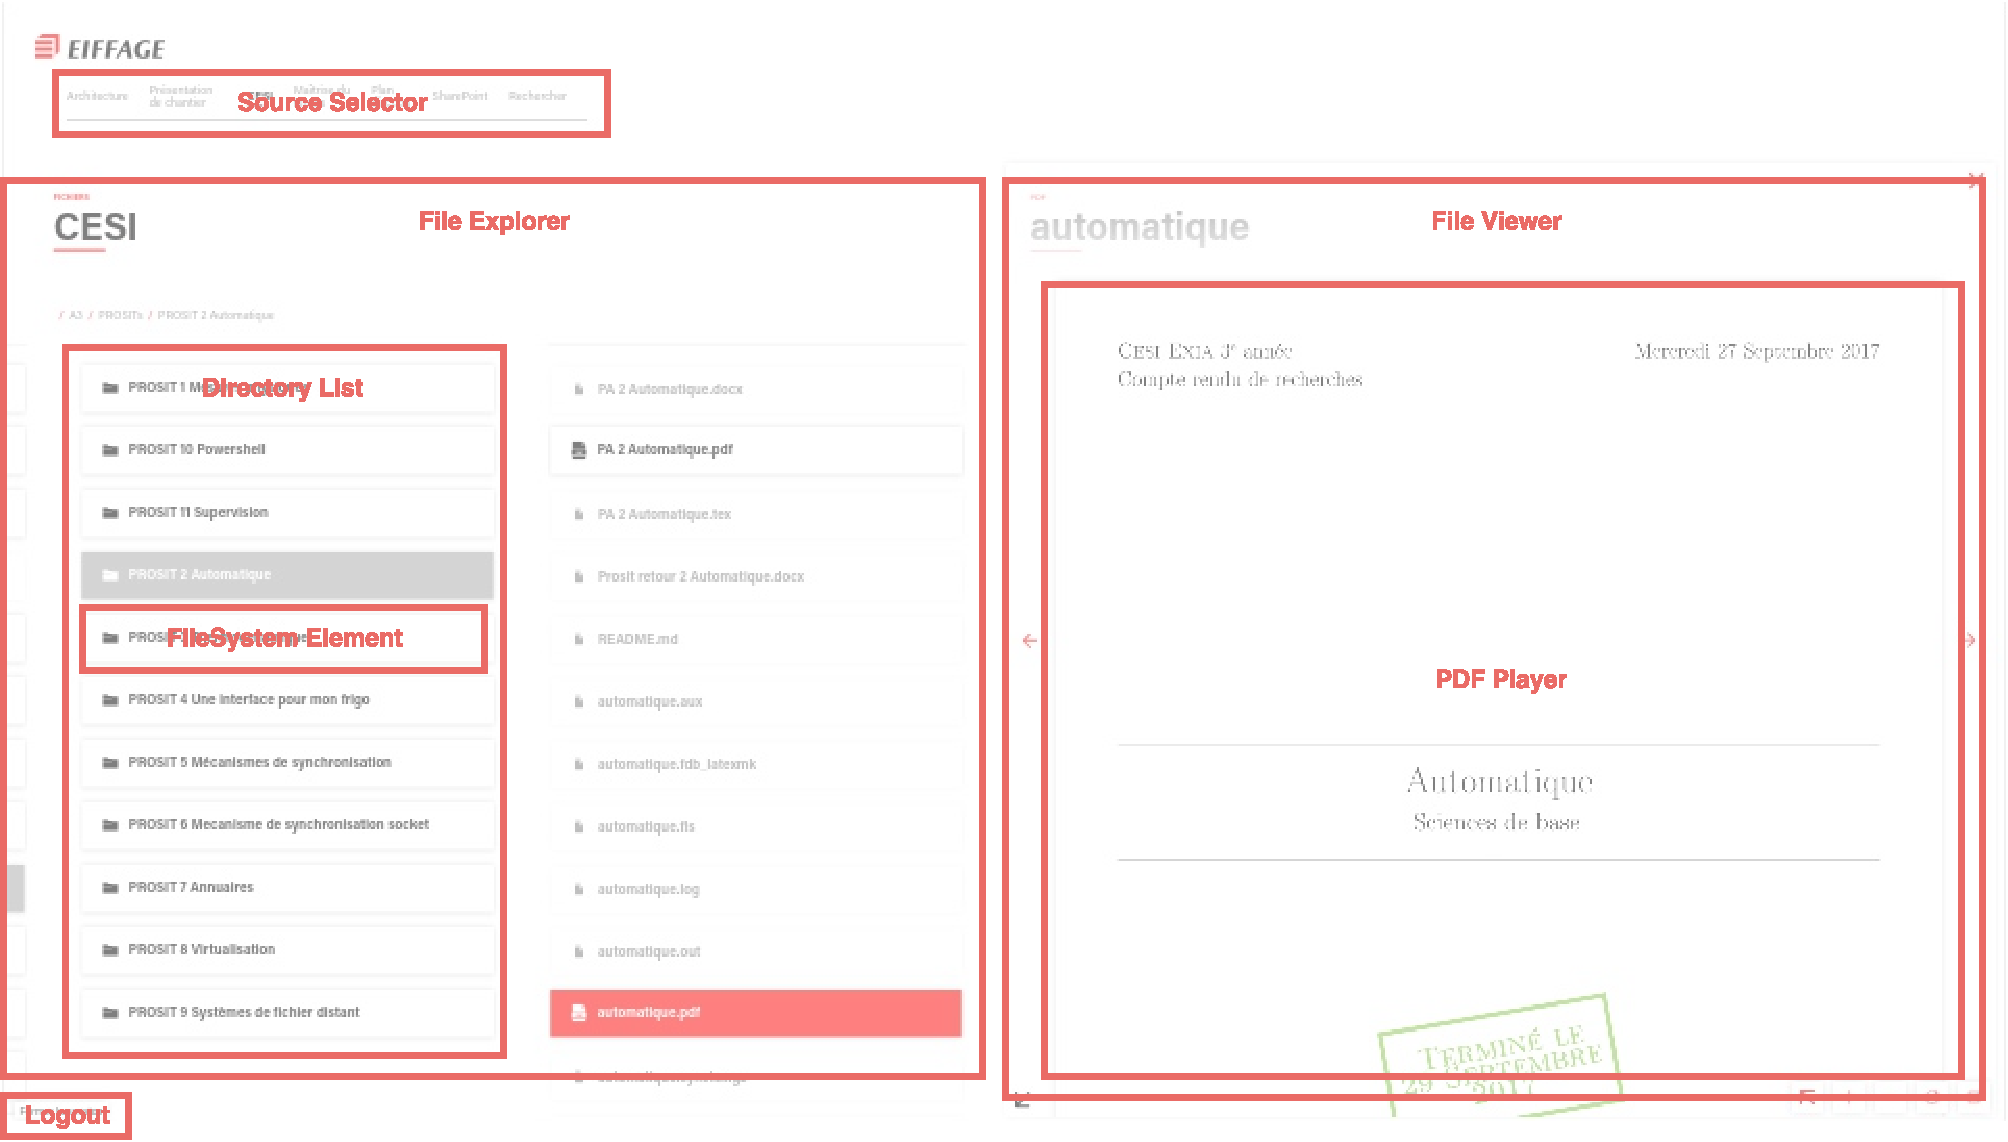
\includegraphics[scale=0.5]{img/media-reader-structure.pdf}
    \caption{La structure de l'application avec les différents components qui composent l'interface}
\end{figure}

Chaque component est séparé des autres et peut fonctionner seul sans nécessiter d'intervention des components parents.

\begin{description}
    \item[Source Selector] Un simple menu de sélection des sources permettant à l'utilisateur de choisir parmi plusieurs éléments disponibles chargés depuis un fichier de configuration général
    \item[File Explorer] Le component principal de l'application, car il permet de naviguer dans les dossiers d'une source et d'ouvrir des fichier  de cette source
    \item[Folder List] Compris dans le component \textbf{File Explorer}, il va lire le contenu d'un dossier passé en attribut et en lister le contenu
    \item[File System Element] Compris dans le component \textbf{Folder List}, ce component va chercher le fichier ou le dossier passer en attribut et afficher son titre et son icône
    \item[File Viewer] Ce component assez simple est en charge d'afficher un aperçu d'un fichier passé en attribut et de choisir le bon lecteur pour le type de fichier demandé
    \item[PDF Player] Le lecteur de fichier, dans ce cas PDF, permettant d'afficher correctement le fichier en fonction de son type; j’ai aussi conçu \texttt{image-player} pour les images et \texttt{video-player} pour les vidéos
    \item[Logout] Un composant conçu par un collègue permettant de se déconnecter de la session Windows actuelle
    \item[Lock Screen] Un component non affiché sur le schéma permettant d'afficher un écran de bienvenue avec un diaporama de photos provenant d'un emplacement réseau en arrière-plan; cet écran de verrouillage s'affiche après une période d'inactivité
    \item[Web Frame] Un composant permettant d'afficher une page Web avec le moteur de rendu webkit
\end{description}

\begin{figure}[h]
    \centering
    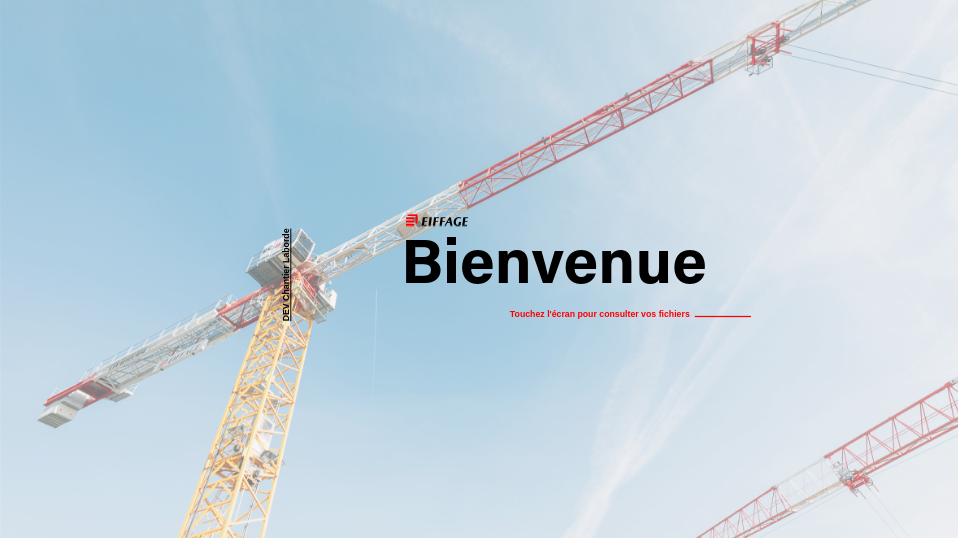
\includegraphics[scale=0.5]{img/media-reader-lock.png}
    \caption{Vue de l'écran de verrouillage du lecteur de médias}
\end{figure}

\subsubsection{Component d'animation}
\label{animationblock}

Les animations prennent une grande place dans le design des applications de LTBL et celles-ci sont prises très au sérieux par l'équipe de développement.
Les animations dans les technologies Web posent quand même un problème.
Elles doivent êtres prises en compte dès la création des éléments pour être correctement utilisables.
De plus l'animation de plusieur éléments les uns a la suite des autres est difficile en CSS.

J'ai donc créé un component Web en charge de gérer les animations.
Un component comme \texttt{Animated Block} permet de ne pas penser à l'animation pendant le développement, mais de l'ajouter à la fin, dès que les fonctionnalités sont ajoutées comme une dernière finition.
Ce component propose un système d'animation se basant sur les transitions CSS (bien plus performantes que les animations JavaScript) et les classes des éléments à animer.

L'\texttt{Animated Block} se présente comme un bloc transparent, qui n'a pas d'incidence sur le style global de l'application.
Il réagit comme un \texttt{div} et peut facilement remplacer un élément de l'interface pour l'animer.

Un \texttt{Animated Block} propose 2 animations par défaut \texttt{enter} et \texttt{leave} servant respectivement a faire apparaître l'élément et a le faire disparaître.
Le component n'impose pas d'animation de base, mais met à disposition système permettant de faire une animation facilement.

Par exemple, prenons l'animation \texttt{enter}.

\begin{figure}[h]
    \centering
    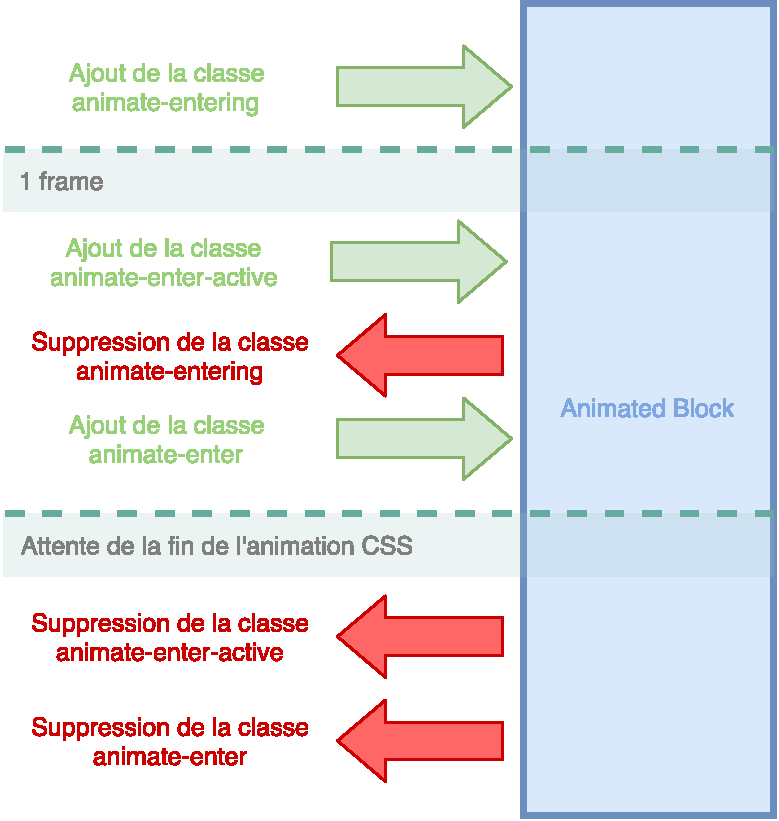
\includegraphics[scale=0.5]{img/animated-block.pdf}
    \caption{Système d'animation d'\texttt{Animated Block}}
\end{figure}

Chaque animation est composée de 3 classes permettant de créer le mouvement correct :

\begin{description}
    \item[Classe de setup] En charge de mettre en style l'élément avant l'animation (Ex. placer l'élément hors de l'écran pour le faire apparaître)
    \item[Classe d'animation] Gérant l'animation dans son ensemble, c'est sur cette classe que l'on positionne la propriété de \texttt{transition} CSS permettant d'animer les différents styles de bloc
    \item[Classe d'état final] En charge de définir l'état final de l'élément après l'animation (elle n'est pas nécessaire si l'état final est le même que l'état standard du bloc)
\end{description}

Ainsi, toute l'animation passe par le fait d'ajouter ou de retirer ces classes.
Le pipeline d'animation est alors le suivant :

\begin{enumerate}
    \item On ajoute la classe de setup (\texttt{animate-entering} dans notre cas)
    \item Une frame plus tard (une fois l'élément stylisé), on ajoute la classe d'animation (\texttt{animate-enter-active} dans notre cas)
    \item On retire la classe de setup puis on ajoute la classe d'état final (\texttt{animate-enter} dans notre cas)
    \item On calcul le temps de l'animation puis on attend la fin de celle-ci
    \item On retire la classe d'animation et d'état final
\end{enumerate}

Il est bien sûr possible de créer ses propres animations en spécifiant manuellement les différentes classes à utiliser, mais les deux animations (\texttt{enter} et \texttt{leave}) sont des animations normalisées.

Dès qu'une animation est déclenchée, une promesse est renvoyée pour permettre de savoir quand elle se terminera.
Cela permet d'effectuer des actions après que l'animation soit passée comme réinitialiser des données ou effectuer des actions en arrière-plan.

Enfin, le component \texttt{Animated Block} dispose d'une fonction statique \texttt{animateStack()} permettant d'animer un ensemble d'éléments les uns après les autres en exécutant simplement une fonction.

Ainsi, grâce à ce système, on peut simplement ajouter des animations au projet sans ajouter beaucoup de lignes de code pouvant mener à des bugs.
Il suffit d'appeler la fonction d'animation et d'attendre la résolution de la promesse pour effectuer des actions après l'animation.

\subsubsection{Submodules Git \& Integration}

Sur les 3 projets que nous avions à développer pour Eiffage, les 3 avaient besoin d'un explorateur de fichier.
Que ce soit pour afficher des aperçus comme le projet actuel ou ouvrir un plan sur la table interactive.
L'explorateur de fichier est un élément essentiel de l'interface.

Et c'est ici que l'on voit l'intérêt d'utiliser des WebComponents.
En effet, il suffit d'utiliser exactement le même code que j'ai utilisé pour le lecteur de médias dans tous les autres projets.

Un autre problème se pose alors.
Il serait contre-productif de faire une copie du code sur chacun des projets et il serait plus intéressant d'utiliser un système de mise à jour automatique.
Cela peut être assuré par les submodules Git.

\begin{figure}[h]
    \centering
    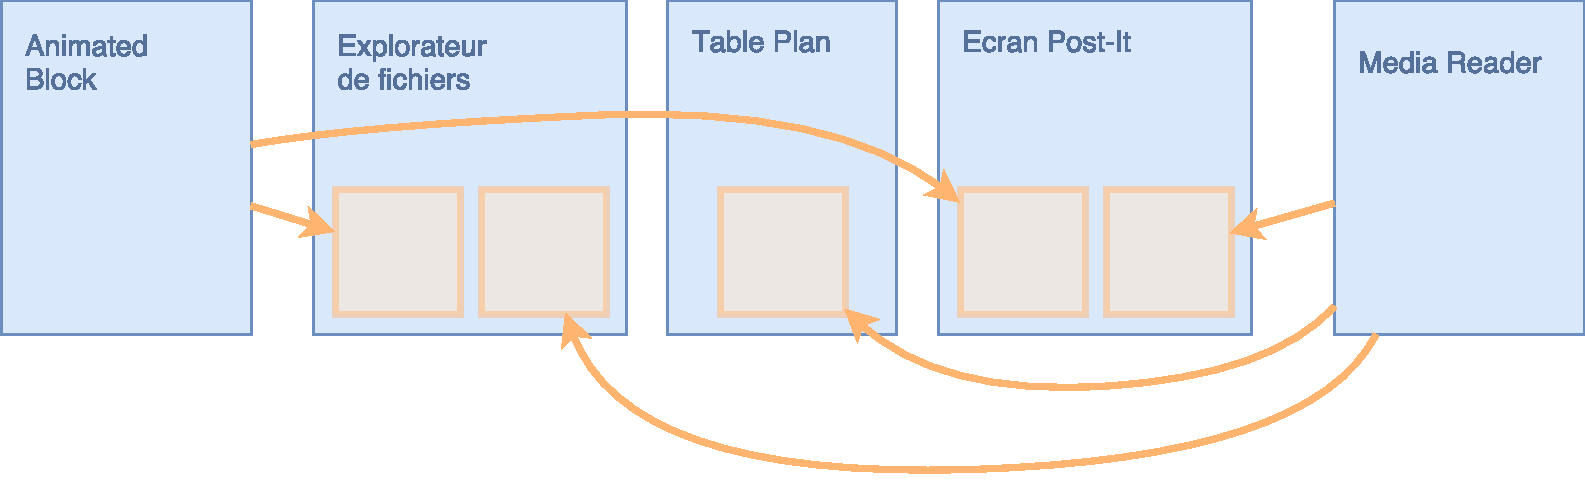
\includegraphics[scale=0.5]{img/submodules.pdf}
    \caption{Exemple d'utilisation des submodules Git}
\end{figure}

Pour tous les projets chez LTBL j'ai utilisé git et BitBucket pour la gestion du code source.
Git dispose d'une fonctionnalité de Submodule.
Cela consiste en un sous-repository dans le projet actuel.
Ce sous-repository fait référence à un repository en ligne commun à tous les projets.

Ainsi, on peut éditer le code du component partagé sur le repository qui lui est dédié puis, sur les projets en ayant besoin, récupérer les modifications avec \texttt{git pull}.

\subsection{Difficultés \& Ergonomie}

Ce projet m'a amené à travailler sur une interface tactile qui allait être utilisée au quotidien et je devais porter une attention toute particulière à l'ergonomie de l'interface.

J'ai alors eu de nombreuses heures d'expérimentations sur les gestes que peuvent avoir les utilisateurs sur les lecteurs comme celui des PDFs .
J'ai ainsi pu me rendre compte de la difficulté d'avoir une réaction ergonomique aux gestes tactiles comme ceux du pincement ou de la rotation à deux doigts.

J'ai donc effectué beaucoup d'expériences avec de nombreux changements de paramètres pour trouver les bonnes valeurs.
Malheureusement, beaucoup de fonctionnalités gestuelles n'ont pas été retenues, car elles n'apportèrent qu'une frustration supplémentaire pour l'utilisateur.

Dans un second temps je me suis aussi heurté au problème des PDF d'Eiffage.
Les plans sont dans ce format et sont générés automatiquement par le logiciel d'architecture.
Il en résulte des documents de très grosse taille et complexe à afficher, ainsi chaque rendu pouvait prendre près de 30 secondes.
Un temps que l'on doit réduire le plus possible pour éviter une attente de la part de l'utilisateur.
Pour réduire ce temps, j'ai mis en place un système qui analyse le zoom effectué et qui ne lance un rendu qu'en cas de zoom important.
Malgré le gain de temps que cela apportait, il fallait trouver une astuce pour éviter les rendus du PDF bien trop lourd.
J'ai alors décidé d'actualiser le zoom du PDF lors du redimensionnement de la fenêtre d'aperçu pour toujours avoir un zoom optimal et réduire le recours au zoom manuel.

\subsection{Installation}

Nous avons installé ce projet sur le site de Laborde près de la garde Saint-Lazare à Paris.
Nous avons installé l'écran de 84 pouces sur son pied et avons installé l'application sur l'ordinateur de manière globale sur la machine.

Un problème s'est posé quand nous avons pris connaissance des pré-requis de sécurité en vogue chez Eiffage.
En effet, Eiffage utilise le système Active Directory et le département Informatique de l'entreprise ne permet pas la création d'un compte spécifique pour l'exécution de l'application.
Il fallait donc faire en sorte que l'application puisse s'exécuter sur n'importe quel utilisateur se connectant.
J'ai alors simplement ajouté un raccourci vers l'application dans le dossier \texttt{Démarrage} du menu démarré global de l'ordinateur pour que l'application se démarre à chaque ouverture de session.
J'ai aussi ajouté un bouton de déconnexion permettant de se déconnecter de la session sans passer par le menu démarrer.

\subsection{Conclusion}

Ce projet m'a permis, au travers d'un sujet simple, de poursuivre ma découverte des WebComponents et des interfaces tactiles.
J'ai rencontré des obstacles qui m'on fait prendre conscience de la difficulté de créer des interfaces tactiles de qualité et le développement de gestes tactiles qui semblent naturels.
Malgré ces problèmes, j'ai réussi à livrer une application fonctionnelle et dont les composants peuvent aisément être intégrés dans les 2 autres projets d'Eiffage qui ont aussi besoin d'un explorateur de fichier.


    \section{Eiffage table plan}
\label{eiffageTablePlan}

%TODO Afficher des plans
\begin{figure}[h]
    \centering
    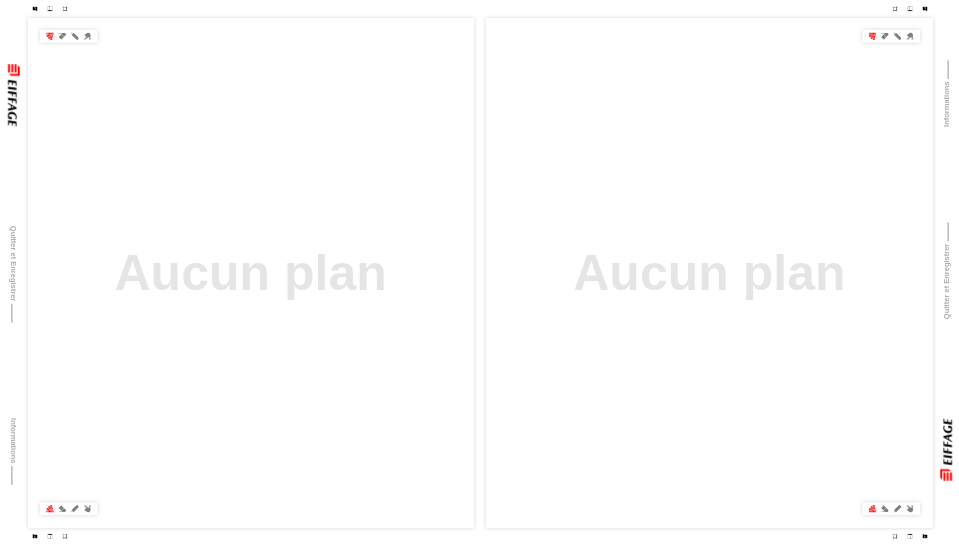
\includegraphics[scale=0.5]{img/table-plan-capture.png}
    \caption{Capture d'écran de l'application Table Plan}
\end{figure}

Dans le trio d'applications de la nouvelle salle cockpit d'Eiffage, l'application d'édition de plan m'a été accordée en partie.
L'objectif de cette application est d'afficher et de permettre la manipulation de plans (au format PDF) issus de  l'espace réseau d'Eiffage.
Cette application est affichée sur un écran intégré dans une table faite sur mesures permettant l'interaction de plusieurs personnes au même moment.

Le cahier des charges de cette application est le suivant :
\begin{itemize}
    \item Charger et afficher des plans depuis le réseau d'Eiffage
    \item Permettre aux utilisateurs de manipuler les plans affichés
    \item Permettre aux utilisateurs d'annoter les plans affichés et d'enregistrer ces annotations pour les transmettre à l'architecte
    \item Utiliser un design compatible avec l'affichage sur une table tactile où plusieurs personnes sont assises autour d'un écran affichant l'application.
\end{itemize}

\subsection{Application existante}
\label{eiffageTablePlanApplicationExistante}

Cette application était la plus avancée des trois lors du début du projet.
L'équipe précédente avait beaucoup travaillé sur l'affichage des PDF .

En effet, les PDF d’ Eiffage sont très lourds et demandent un affichage particulier.
L'équipe ayant travaillé sur ce projet a donc beaucoup réfléchi à la technologie à utiliser pour afficher les PDF sans ralentissement.
Ils ont donc opté pour une approche orientée Web avec un chargement, non pas du PDF en lui même, mais d'une image de ce PDF rendue à l'aide de ImageMagick.
Ils ont alors utilisé PixiJs, une librairie 2D pour WebGL, pour afficher l'image du PDF et permettre l'annotation.

Le plus gros de l'application, l'édition de plan était déjà codée et j'ai donc eu l'objectif de créer l'interface pour qu'elle reflète les créations du designer.
Mais aussi que l'application soit utilisable en collaboration et donc autour d'une table.

En revanche, l'ancienne application n'utilisait pas les WebComponents et j'ai dû m'adapter pour reformer le code présent.
De plus, le développeur me précédent, n'avait pas du tout les mêmes habitudes de développement et la même structure que moi et j'ai donc eu une longue phase d'analyse pour comprendre le rôle de chaque élément.

\subsection{Technologie}
\label{eiffageTablePlanTechnologie}

Les technologies utilisées dans le cadre de ce projet sont les mêmes que les autres applications de ce type créent par LTBL.
On y retrouve Electron pour l'affichage de l'application et les WebComponents pour la structure interne.

\subsection{Structure}
\label{eiffageTablePlanStructure}

L'application se divise alors en de multiples WebComponents chacun ayant un rôle spécifique.

\begin{figure}[h]
    \centering
    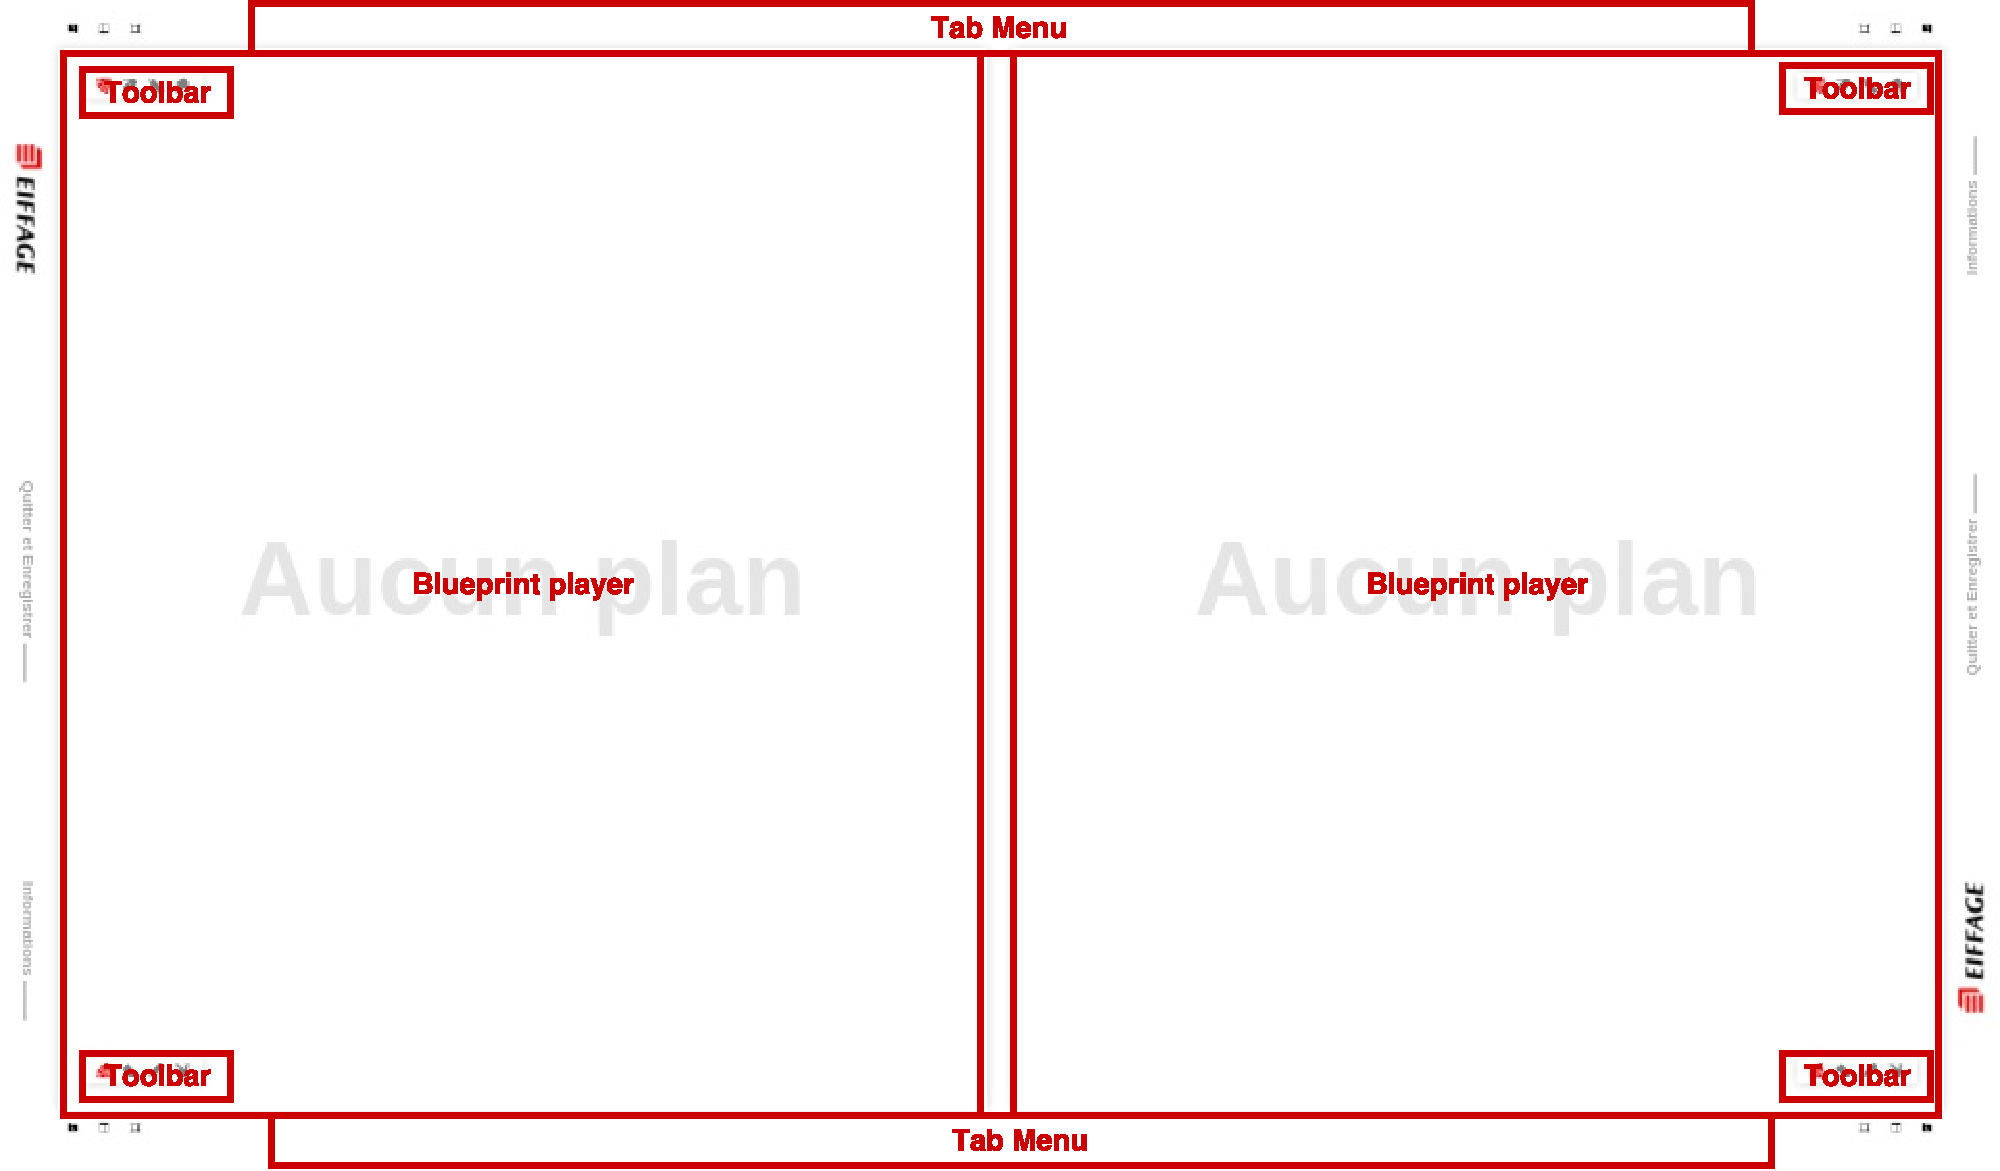
\includegraphics[scale=0.5]{img/table-plan-structure.pdf}
    \caption{Structure de l'application Table Plan}
\end{figure}

On retrouve alors les composants suivants

\paragraph{Blueprint player} Un component en charge d'afficher et d'annoter un plan dans notre cas.
Ce component était déjà, en grande partie, conçu quand j'ai débuté le développement de l'interface.
Anisi, je n'ai eu qu'à l'intégrer dans l'application finale.

\paragraph{Tab menu} Le menu composé de différents onglets.
Chaque onglet représente un plan ouvert qui peut être affiché.
Ce component est présent en 2 exemplaires dont un retourné sur le haut de l'application destiné aux utilisateurs présents de l'autre côté de la table.
J'ai synchronisé l'état de ces deux components avec un système de Store (\emph{cf} partie\ref{eiffageTablePlanStores})

\paragraph{Toolbar} Un composant affichant divers boutons permettant de choisir l'outil à utiliser dans sur le plan affiché.
Ce component est présent en 4 exemplaires dans l'application et doit donc être synchronisé avec ses voisins.
J'ai aussi utilisé le système de store pour synchroniser les états des barres d'outils et des éditeurs de plans (\texttt{Blueprint Player}).

\bigskip

Dans cette application, j'ai aussi utilisé le component \texttt{Media reader} du projet précédent pour offrir une interface unifiée sur toutes les applications développées pour Eiffage.
Je l'ai ajouté par le biais des submodules Git et de quelques petits ajustements dans le code de base de l'explorateur.

\subsection{Style}
\label{eiffageTablePlanStyle}

L'un des points majeurs de cette mission fut le style de l'application.
En effet, on est loin d'une application standard exécutée sur un bureau.
On remarque que l'utilisation faite de cette application nécessite une mise en place particulière des éléments de l'interface.

On remarque notamment que les barres d'outils sont présentes aux 4 coins de l'interface toutes dirigés vers l'extérieur de l'application pour permettre an'importe quel collaborateur autour de la table d'interagir avec les plans.
Cela a demandé la mise en place d'une synchronisation des barres d'outils au niveau de l'application et l'utilisation de propriétés CSS de transformations a des fins bien plus ergonomiques qu'esthétiques.

\bigskip

On remarque aussi que la barre des onglets ouverts est aussi inversée sur la partie supérieure de l'application.
Cela a demandé une modification au niveau du code lui-même, car je ne pouvais pas me contenter d'effectuer un miroir sur l'élément (ce que j'ai fait pour les barres d'outils).
La raison de cette spécificité est la présence de texte.
Mettre un effet de miroir sur un texte le rend complètement illisible (contrairement à une icône) et j'ai effectué une rotation au lieu de faire un miroir.
Mais cela posé d'autres problèmes puisque la droite et la gauche était inverse sur chacun des éléments.
J'ai donc modifié le code source du composant de la barre d'onglets pour qu'elle inverse toutes les commandes dans certains cas.

\subsection{Stockage de données}
\label{eiffageTablePlanStores}

Par son style particulier et la dimension collaborative de la table, de nombreux éléments de l'interface doivent être synchronisés.
Par exemple, il faut synchroniser l'état des barres tout'ils pour qu'elles affichent en tout temps le bon outil en cours d'utilisation même si cet outil est changé depuis un élément extérieur comme une autre barre d'outils.

J'ai, dans un premier temps, imaginé un système inclus dans les components permettant de les lier directement pour qu'ils s'informent entre eux lors d'un changement d'état d'un côté.

\begin{figure}[h]
    \centering
    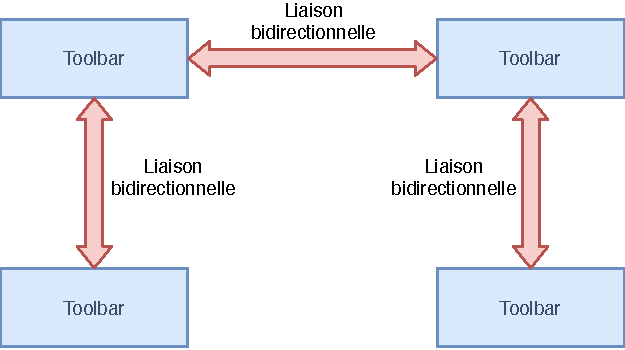
\includegraphics[scale=1]{img/premiere-synchro.pdf}
    \caption{Premier système de synchronisation utilisé dans le cas des barres d'outils de l'application}
\end{figure}

Cela fonctionnait, mais je me suis vite heurté à la rigidité de ce système et à la complexité d'étendre les fonctionnalités de ce système à l'application entière.
J'ai donc puisé dans mes connaissances et me suis inspiré des solutions trouvées dans des librairies comme \emph{Vuex} pour concevoir les Stores.

Un store est une classe Singleton\footnote{Une classe qui ne peut être instanciée qu'une seule fois et accessible par tout le programme}  qui va stocker un état particulier.
Cette classe est observable et peut donc informer les éléments de l'interface qui lui sont abonnés des changements apportés à l'état du store.
Ce système permet de centraliser la gestion des informations à l'échelle de l'application sans pour autant rendre les components dépendants les uns des autres.
De plus, ce système permet une grande flexibilité, car on peut modifier l'état à n'importe quel endroit de l'interface.
Ces changements seront alors répercutés sur l'ensemble de l'application automatiquement et dynamiquement.

\begin{figure}[h]
    \centering
    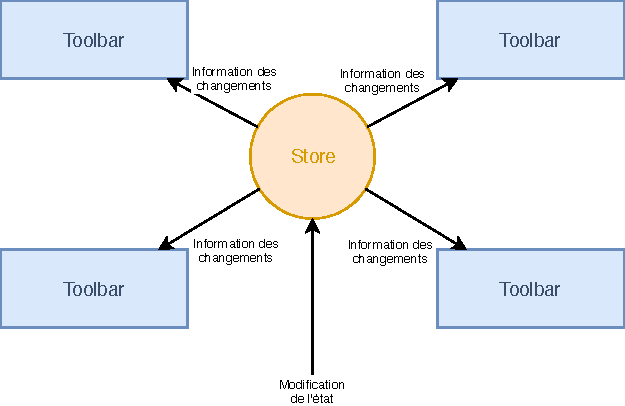
\includegraphics[scale=1.5]{img/store.pdf}
    \caption{Le fonctionnement du store dans le cadre de la gestion des barres d'outils}
\end{figure}

J'ai alors réutilisé ce système dans la gestion des plans ouverts et en cours de conversion (\emph{cf} partie \ref{eiffageTablePlanConversion}) sur Tableplan.
Mais aussi dans les autres applications que j'ai été amené à développer à la suite de celle-ci.

\clearpage

\subsection{Conversion}
\label{eiffageTablePlanConversion}

Les plans d'Eiffage étant très lourds, ils sont impossibles à ouvrir tel quel dans l'application.
Il faut donc utiliser un logiciel de conversion pour rendre les PDF sous forme d'image.

Les PDF de plans d'Eiffage étant des plans vectoriels\footnote{Une image vectorielle est une image dont on ne spécifie pas la couleur de chaque pixel, mais on spécifie une suite d'instruction permettant de calculer l'image finale. Les fichiers PDF, AI et SVG sont des exemples de fichiers vectoriels} Ils nécessitent un calcul préalable pour les afficher.
Pour résoudre le problème de lourdeur des fichiers, j'ai mis en place un système de conversion automatique des plans.

\bigskip

Dès qu'un fichier PDF est ouvert, on vérifie dans un dossier de cache s'il n'est pas déjà converti.
S’ il l'est, on ouvre simplement la conversion précédente.
S'il ne l'est pas, on lance une conversion.
On informa alors l'utilisateur de la conversion en cours et on attend la fin de cette conversion avant d'ouvrir le fichier converti.

\begin{figure}[h]
    \centering
    
\includegraphics[scale=0.3]{img/image-magick.png}
    \hspace{5cm}
    
\includegraphics[scale=0.13]{img/ghostscript.png}
    \caption{Les logis de ImageMagick (à gauche) et GhostScript (à droite)}
\end{figure}

La conversion est effectuée avec ImageMagick, un logiciel de manipulation d'images très performant, et de GhostScript, un logiciel permettant de rendre des fichiers PDF avec ImageMagick.

Pour permettre un rendu optimal dans toutes les circonstances, nous avons choisi de rendre les plans en 4K et de les afficher dans une fenêtre 4 fois supérieure à leur taille pour avoir un trait d'annotation fin bien défini.

\subsection{Conclusion}
\label{eiffageTablePlanConclusion}

Ce projet fut pour moi l'occasion d'expérimenter plus en profondeur les stockages des données au sein d'une application basée sur des composants.
Ce fut aussi une bonne expérience de travail en équipe, car je n'ai développé que l'interface qui entourait un système d'affichage et d'annotation de plans développé par le reste de l'équipe.


    \section{Biopedia BioMérieux}

    \section{Bilan}

    \section{Conclusion}

\end{document}
